% Options for packages loaded elsewhere
% Options for packages loaded elsewhere
\PassOptionsToPackage{unicode}{hyperref}
\PassOptionsToPackage{hyphens}{url}
\PassOptionsToPackage{dvipsnames,svgnames,x11names}{xcolor}
%
\documentclass[
  letterpaper,
]{article}
\usepackage{xcolor}
\usepackage{amsmath,amssymb}
\setcounter{secnumdepth}{5}
\usepackage{iftex}
\ifPDFTeX
  \usepackage[T1]{fontenc}
  \usepackage[utf8]{inputenc}
  \usepackage{textcomp} % provide euro and other symbols
\else % if luatex or xetex
  \usepackage{unicode-math} % this also loads fontspec
  \defaultfontfeatures{Scale=MatchLowercase}
  \defaultfontfeatures[\rmfamily]{Ligatures=TeX,Scale=1}
\fi
\usepackage{lmodern}
\ifPDFTeX\else
  % xetex/luatex font selection
\fi
% Use upquote if available, for straight quotes in verbatim environments
\IfFileExists{upquote.sty}{\usepackage{upquote}}{}
\IfFileExists{microtype.sty}{% use microtype if available
  \usepackage[]{microtype}
  \UseMicrotypeSet[protrusion]{basicmath} % disable protrusion for tt fonts
}{}
\makeatletter
\@ifundefined{KOMAClassName}{% if non-KOMA class
  \IfFileExists{parskip.sty}{%
    \usepackage{parskip}
  }{% else
    \setlength{\parindent}{0pt}
    \setlength{\parskip}{6pt plus 2pt minus 1pt}}
}{% if KOMA class
  \KOMAoptions{parskip=half}}
\makeatother
% Make \paragraph and \subparagraph free-standing
\makeatletter
\ifx\paragraph\undefined\else
  \let\oldparagraph\paragraph
  \renewcommand{\paragraph}{
    \@ifstar
      \xxxParagraphStar
      \xxxParagraphNoStar
  }
  \newcommand{\xxxParagraphStar}[1]{\oldparagraph*{#1}\mbox{}}
  \newcommand{\xxxParagraphNoStar}[1]{\oldparagraph{#1}\mbox{}}
\fi
\ifx\subparagraph\undefined\else
  \let\oldsubparagraph\subparagraph
  \renewcommand{\subparagraph}{
    \@ifstar
      \xxxSubParagraphStar
      \xxxSubParagraphNoStar
  }
  \newcommand{\xxxSubParagraphStar}[1]{\oldsubparagraph*{#1}\mbox{}}
  \newcommand{\xxxSubParagraphNoStar}[1]{\oldsubparagraph{#1}\mbox{}}
\fi
\makeatother

\usepackage{color}
\usepackage{fancyvrb}
\newcommand{\VerbBar}{|}
\newcommand{\VERB}{\Verb[commandchars=\\\{\}]}
\DefineVerbatimEnvironment{Highlighting}{Verbatim}{commandchars=\\\{\}}
% Add ',fontsize=\small' for more characters per line
\usepackage{framed}
\definecolor{shadecolor}{RGB}{241,243,245}
\newenvironment{Shaded}{\begin{snugshade}}{\end{snugshade}}
\newcommand{\AlertTok}[1]{\textcolor[rgb]{0.68,0.00,0.00}{#1}}
\newcommand{\AnnotationTok}[1]{\textcolor[rgb]{0.37,0.37,0.37}{#1}}
\newcommand{\AttributeTok}[1]{\textcolor[rgb]{0.40,0.45,0.13}{#1}}
\newcommand{\BaseNTok}[1]{\textcolor[rgb]{0.68,0.00,0.00}{#1}}
\newcommand{\BuiltInTok}[1]{\textcolor[rgb]{0.00,0.23,0.31}{#1}}
\newcommand{\CharTok}[1]{\textcolor[rgb]{0.13,0.47,0.30}{#1}}
\newcommand{\CommentTok}[1]{\textcolor[rgb]{0.37,0.37,0.37}{#1}}
\newcommand{\CommentVarTok}[1]{\textcolor[rgb]{0.37,0.37,0.37}{\textit{#1}}}
\newcommand{\ConstantTok}[1]{\textcolor[rgb]{0.56,0.35,0.01}{#1}}
\newcommand{\ControlFlowTok}[1]{\textcolor[rgb]{0.00,0.23,0.31}{\textbf{#1}}}
\newcommand{\DataTypeTok}[1]{\textcolor[rgb]{0.68,0.00,0.00}{#1}}
\newcommand{\DecValTok}[1]{\textcolor[rgb]{0.68,0.00,0.00}{#1}}
\newcommand{\DocumentationTok}[1]{\textcolor[rgb]{0.37,0.37,0.37}{\textit{#1}}}
\newcommand{\ErrorTok}[1]{\textcolor[rgb]{0.68,0.00,0.00}{#1}}
\newcommand{\ExtensionTok}[1]{\textcolor[rgb]{0.00,0.23,0.31}{#1}}
\newcommand{\FloatTok}[1]{\textcolor[rgb]{0.68,0.00,0.00}{#1}}
\newcommand{\FunctionTok}[1]{\textcolor[rgb]{0.28,0.35,0.67}{#1}}
\newcommand{\ImportTok}[1]{\textcolor[rgb]{0.00,0.46,0.62}{#1}}
\newcommand{\InformationTok}[1]{\textcolor[rgb]{0.37,0.37,0.37}{#1}}
\newcommand{\KeywordTok}[1]{\textcolor[rgb]{0.00,0.23,0.31}{\textbf{#1}}}
\newcommand{\NormalTok}[1]{\textcolor[rgb]{0.00,0.23,0.31}{#1}}
\newcommand{\OperatorTok}[1]{\textcolor[rgb]{0.37,0.37,0.37}{#1}}
\newcommand{\OtherTok}[1]{\textcolor[rgb]{0.00,0.23,0.31}{#1}}
\newcommand{\PreprocessorTok}[1]{\textcolor[rgb]{0.68,0.00,0.00}{#1}}
\newcommand{\RegionMarkerTok}[1]{\textcolor[rgb]{0.00,0.23,0.31}{#1}}
\newcommand{\SpecialCharTok}[1]{\textcolor[rgb]{0.37,0.37,0.37}{#1}}
\newcommand{\SpecialStringTok}[1]{\textcolor[rgb]{0.13,0.47,0.30}{#1}}
\newcommand{\StringTok}[1]{\textcolor[rgb]{0.13,0.47,0.30}{#1}}
\newcommand{\VariableTok}[1]{\textcolor[rgb]{0.07,0.07,0.07}{#1}}
\newcommand{\VerbatimStringTok}[1]{\textcolor[rgb]{0.13,0.47,0.30}{#1}}
\newcommand{\WarningTok}[1]{\textcolor[rgb]{0.37,0.37,0.37}{\textit{#1}}}

\usepackage{longtable,booktabs,array}
\usepackage{calc} % for calculating minipage widths
% Correct order of tables after \paragraph or \subparagraph
\usepackage{etoolbox}
\makeatletter
\patchcmd\longtable{\par}{\if@noskipsec\mbox{}\fi\par}{}{}
\makeatother
% Allow footnotes in longtable head/foot
\IfFileExists{footnotehyper.sty}{\usepackage{footnotehyper}}{\usepackage{footnote}}
\makesavenoteenv{longtable}
\usepackage{graphicx}
\makeatletter
\newsavebox\pandoc@box
\newcommand*\pandocbounded[1]{% scales image to fit in text height/width
  \sbox\pandoc@box{#1}%
  \Gscale@div\@tempa{\textheight}{\dimexpr\ht\pandoc@box+\dp\pandoc@box\relax}%
  \Gscale@div\@tempb{\linewidth}{\wd\pandoc@box}%
  \ifdim\@tempb\p@<\@tempa\p@\let\@tempa\@tempb\fi% select the smaller of both
  \ifdim\@tempa\p@<\p@\scalebox{\@tempa}{\usebox\pandoc@box}%
  \else\usebox{\pandoc@box}%
  \fi%
}
% Set default figure placement to htbp
\def\fps@figure{htbp}
\makeatother





\setlength{\emergencystretch}{3em} % prevent overfull lines

\providecommand{\tightlist}{%
  \setlength{\itemsep}{0pt}\setlength{\parskip}{0pt}}



 


\usepackage{orcidlink}  
\usepackage[nonatbib, final]{neurips_2023}
\usepackage{amsmath}
\usepackage{amsthm}
\usepackage[utf8]{inputenc} % allow utf-8 input
\usepackage[T1]{fontenc}    % use 8-bit T1 fonts
\usepackage{hyperref}       % hyperlinks
\usepackage{url}            % simple URL typesetting
\usepackage{booktabs}       % professional-quality tables
\usepackage{amsfonts}       % blackboard math symbols
\usepackage{nicefrac}       % compact symbols for 1/2, etc.
\usepackage{microtype}      % microtypography
\usepackage{xcolor}         % colors
\usepackage[numbers]{natbib}
\usepackage{comment}
\usepackage{graphicx} 
\bibliographystyle{abbrvnat}
\makeatletter
\@ifpackageloaded{caption}{}{\usepackage{caption}}
\AtBeginDocument{%
\ifdefined\contentsname
  \renewcommand*\contentsname{Table of contents}
\else
  \newcommand\contentsname{Table of contents}
\fi
\ifdefined\listfigurename
  \renewcommand*\listfigurename{List of Figures}
\else
  \newcommand\listfigurename{List of Figures}
\fi
\ifdefined\listtablename
  \renewcommand*\listtablename{List of Tables}
\else
  \newcommand\listtablename{List of Tables}
\fi
\ifdefined\figurename
  \renewcommand*\figurename{Figure}
\else
  \newcommand\figurename{Figure}
\fi
\ifdefined\tablename
  \renewcommand*\tablename{Table}
\else
  \newcommand\tablename{Table}
\fi
}
\@ifpackageloaded{float}{}{\usepackage{float}}
\floatstyle{ruled}
\@ifundefined{c@chapter}{\newfloat{codelisting}{h}{lop}}{\newfloat{codelisting}{h}{lop}[chapter]}
\floatname{codelisting}{Listing}
\newcommand*\listoflistings{\listof{codelisting}{List of Listings}}
\makeatother
\makeatletter
\makeatother
\makeatletter
\@ifpackageloaded{caption}{}{\usepackage{caption}}
\@ifpackageloaded{subcaption}{}{\usepackage{subcaption}}
\makeatother
\usepackage{bookmark}
\IfFileExists{xurl.sty}{\usepackage{xurl}}{} % add URL line breaks if available
\urlstyle{same}
\hypersetup{
  pdftitle={Adaptive Book Imbalance Execution Strategies Lead to Robust Improvements Over Naive Benchmark},
  pdfauthor={Michael Cusack-Nelkin; Alick Zhou; Debby Zhao; Michael Bakshandeh; Vijeet Prasad},
  pdfkeywords={optimal, execution, order, splitting, imbalance},
  colorlinks=true,
  linkcolor={blue},
  filecolor={Maroon},
  citecolor={Blue},
  urlcolor={Blue},
  pdfcreator={LaTeX via pandoc}}



\title{Adaptive Book Imbalance Execution Strategies Lead to Robust
Improvements Over Naive Benchmark}
\author{
\textbf{Michael Cusack-Nelkin}%
\\%
%
\texttt{mc5882@columbia.edu}\and 
\textbf{Alick Zhou}%
\\%
%
\texttt{az2960@columbia.edu}\and 
\textbf{Debby Zhao}%
\\%
%
\texttt{lz3083@columbia.edu}\and 
\textbf{Michael Bakshandeh}%
\\%
%
\texttt{mb5499@columbia.edu}\and 
\textbf{Vijeet Prasad}%
\\%
%
\texttt{vp2580@columbia.edu}}
\date{2026-05-19}
\begin{document}
\maketitle
\begin{abstract}
A fundamental challenge in medium-frequency systematic trading is the
underperformance of simple execution strategies. Naively splitting a
parent order into smaller market-orders over seconds or minutes exposes
child fills to adverse price drifts, and can also lead to large price
impact. In this work we compare the arrival cost of different order
splitting and execution strategies from the naive zero-intelligence to
the dynamically adaptive, with the goal of reducing the total arrival
cost of a parent order, subject to time, quantity, and price
constraints. To do this, we use level two orderbook data sourced from
Databento, and build an order book simulation capable of simulating the
fills and price impact of any arbitrary execution strategy using common
order types. We examine three failed execution strategies and their
individual advancements and issues. We showcase our final
implementation, which achieves robust cost reductions of 55\% - 89\%, by
intelligently calibrating the aggression of child orders to take
advantage of favorable price conditions while avoiding unfavorable ones.
We then examine this strategy's mechanics, results and statistical
significance for three assets and for ranges of latency and book
replenishment parameters. Finally, we suggest further tweaks and
improvements to the strategy, to be pursued in the future.
\end{abstract}


\section{Motivation and Main Ideas}\label{motivation-and-main-ideas}

\subsection{Underperformance of Naive
Splitting}\label{underperformance-of-naive-splitting}

The main driver of this work is the unfortunate underperformance of
simple execution strategies. Naively splitting a parent order into \(n\)
chunks and filling them as market orders \(\Delta t\) time units apart
has high impact and exposes the parent order to significant price
drifts. Figure~\ref{fig-naive} shows the price impact of repeatedly
lifting the ask over time. This simulated fill split a 5000-share buy
order into twenty-five 200-share fills. The underperformance of this
strategy necessitates a more intelligent way to identify favorable ways
to fill and split large orders.

\subsection{Book Imbalance as a Primary
Signal}\label{book-imbalance-as-a-primary-signal}

The core of our improvements over the naive method make use of the
imbalance in quantity on the top six levels of the book as a predictive
signal over short horizons. Structurally, as marketable buy and sell
orders arrive at approximately equal rates, imbalance in top of book
depth should predict which levels are depleted fastest and therefore the
direction of a subsequent price movement. We chose OBI because it is a
well understood, easy to implement, and powerful signal of price
direction on the micro-to-milli-second time scale. As evidence of OBI's
predictive power, we used the markout plot in Figure~\ref{fig-markout}.
Within five separate ranges of OBI values, we sample 100,000 timestamps
and calculate the difference between the initial mid-price and the
mid-price at 10,000 subsequent times, then average over each of the
100,000 paths. We use a time horizon of \([0,10]\) milliseconds, in
steps of ten microseconds.

\begin{figure}

\begin{minipage}{0.50\linewidth}

\begin{figure}[H]

\centering{

\pandocbounded{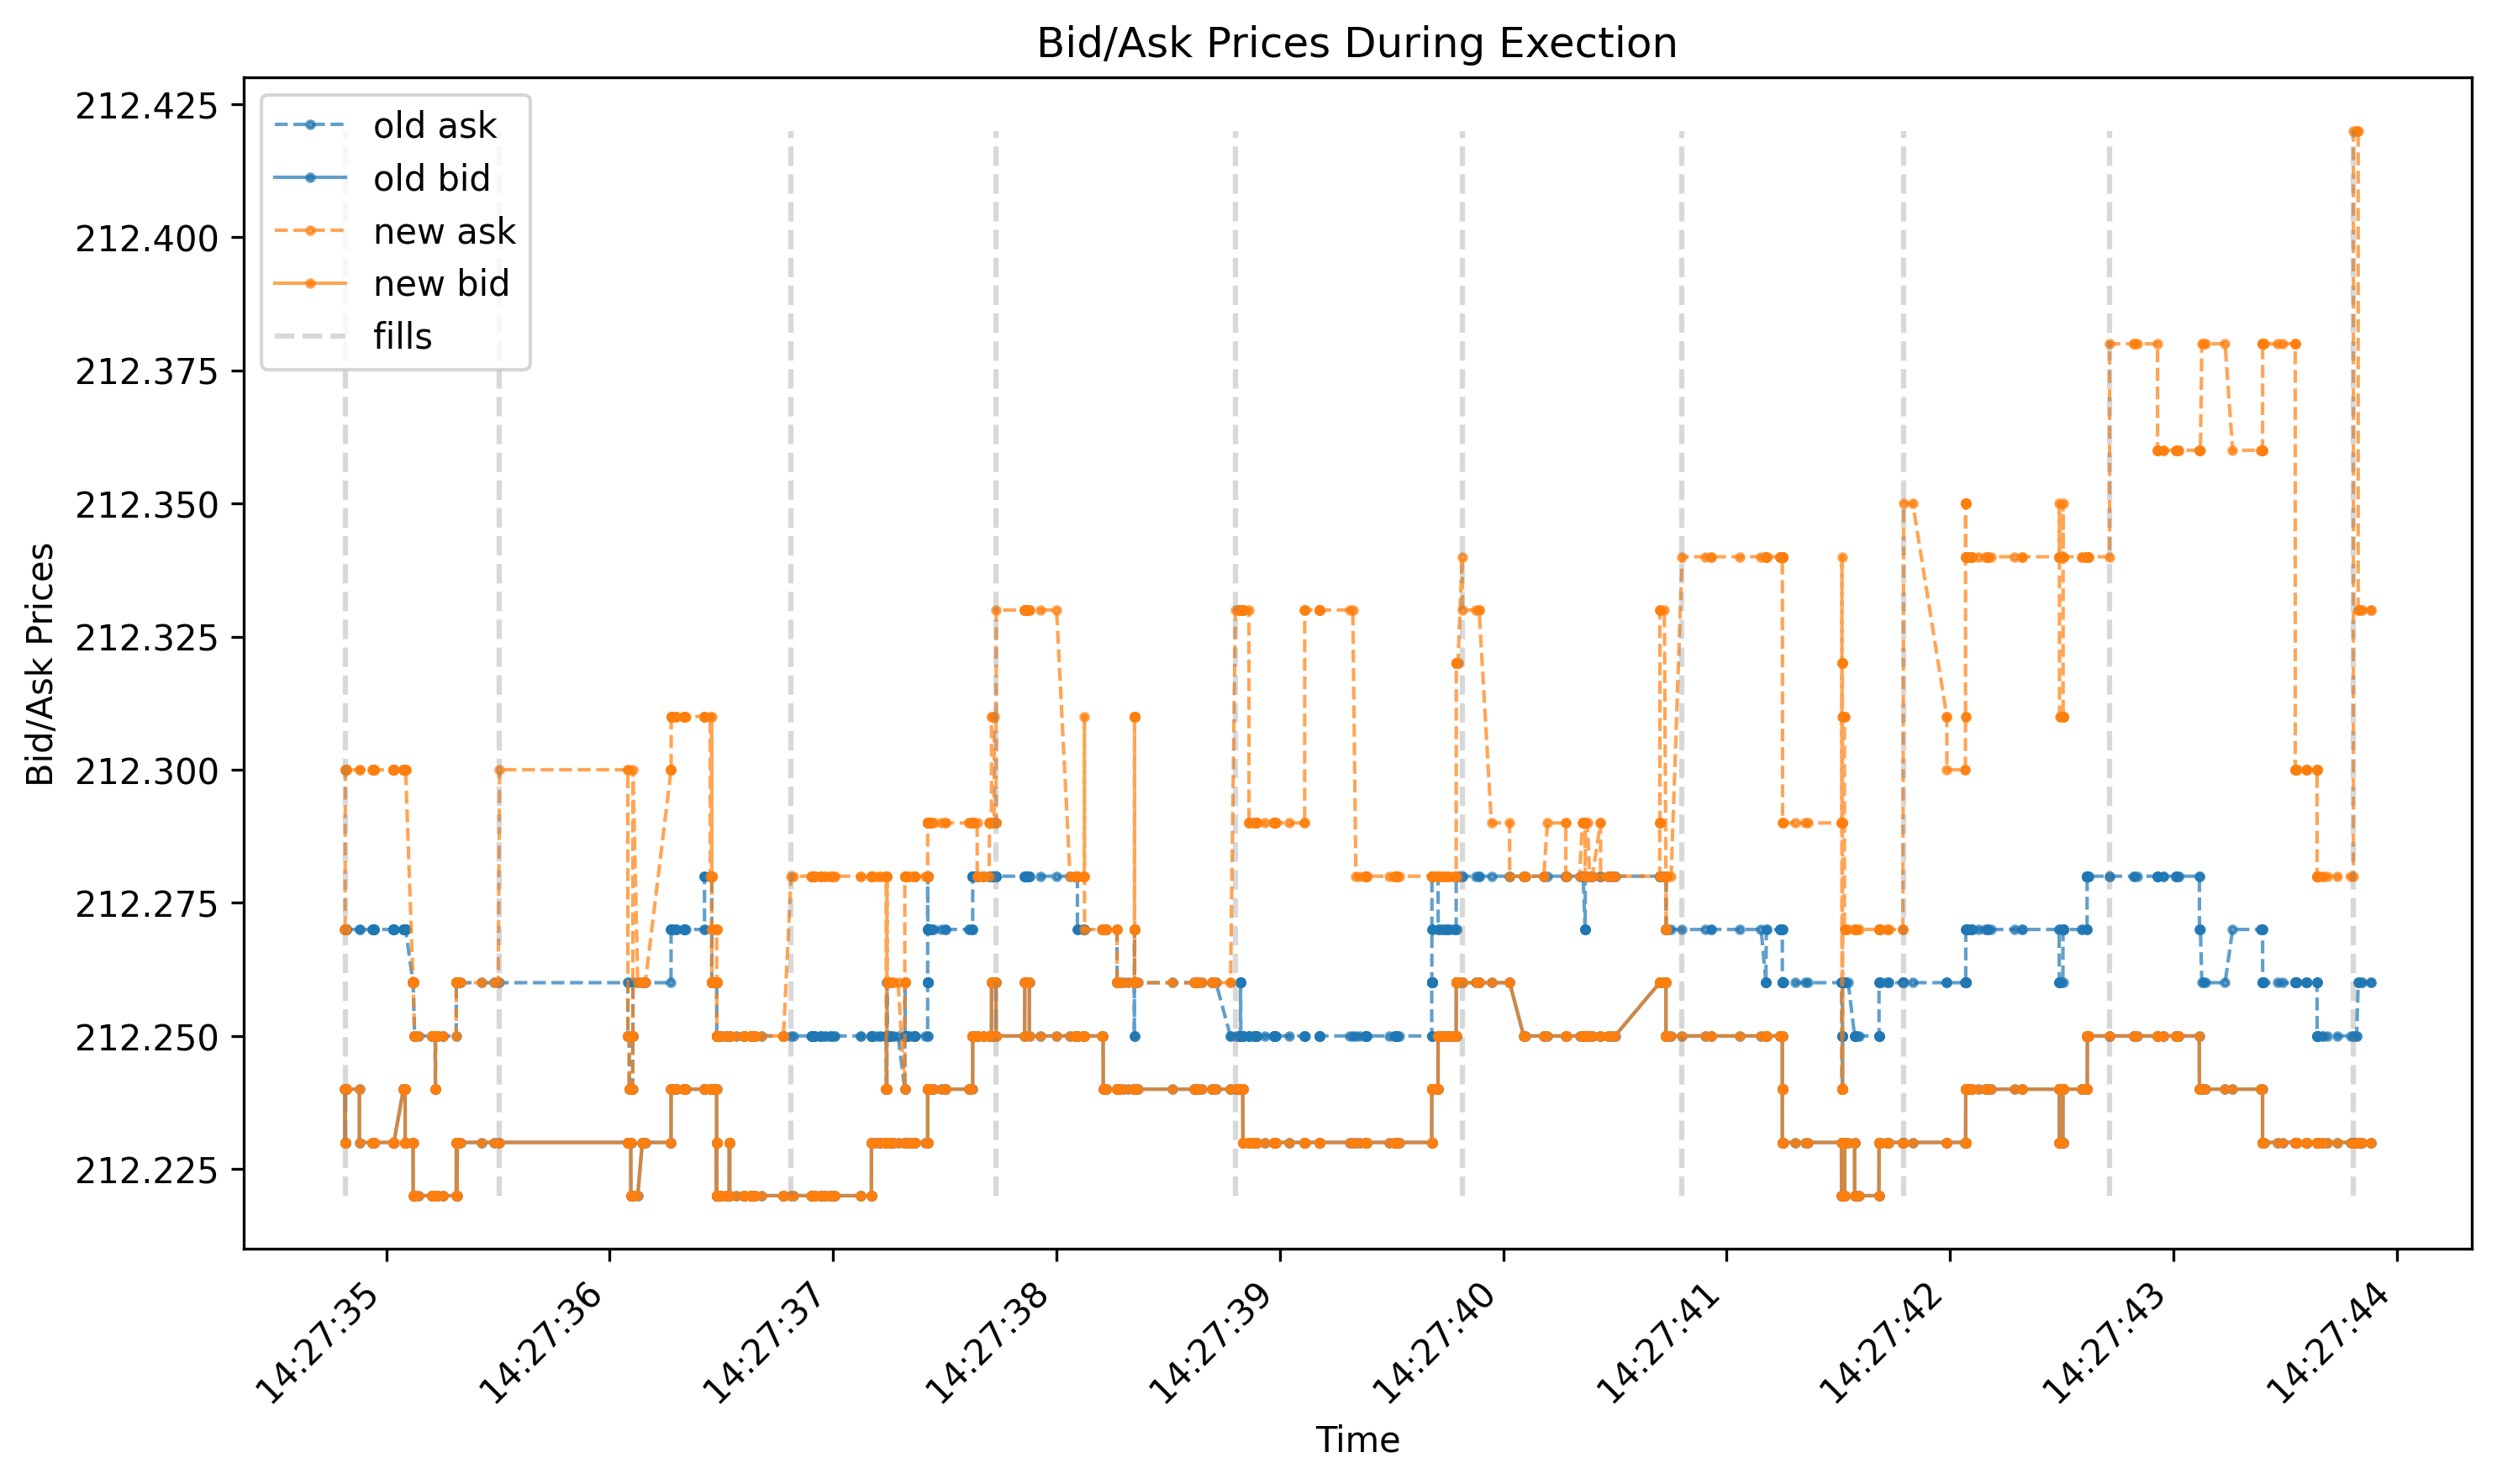
\includegraphics[keepaspectratio]{plots_and_data/section_1/naive.png}}

}

\caption{\label{fig-naive}Naive Order Splitting}

\end{figure}%

\end{minipage}%
%
\begin{minipage}{0.50\linewidth}

\begin{figure}[H]

\centering{

\pandocbounded{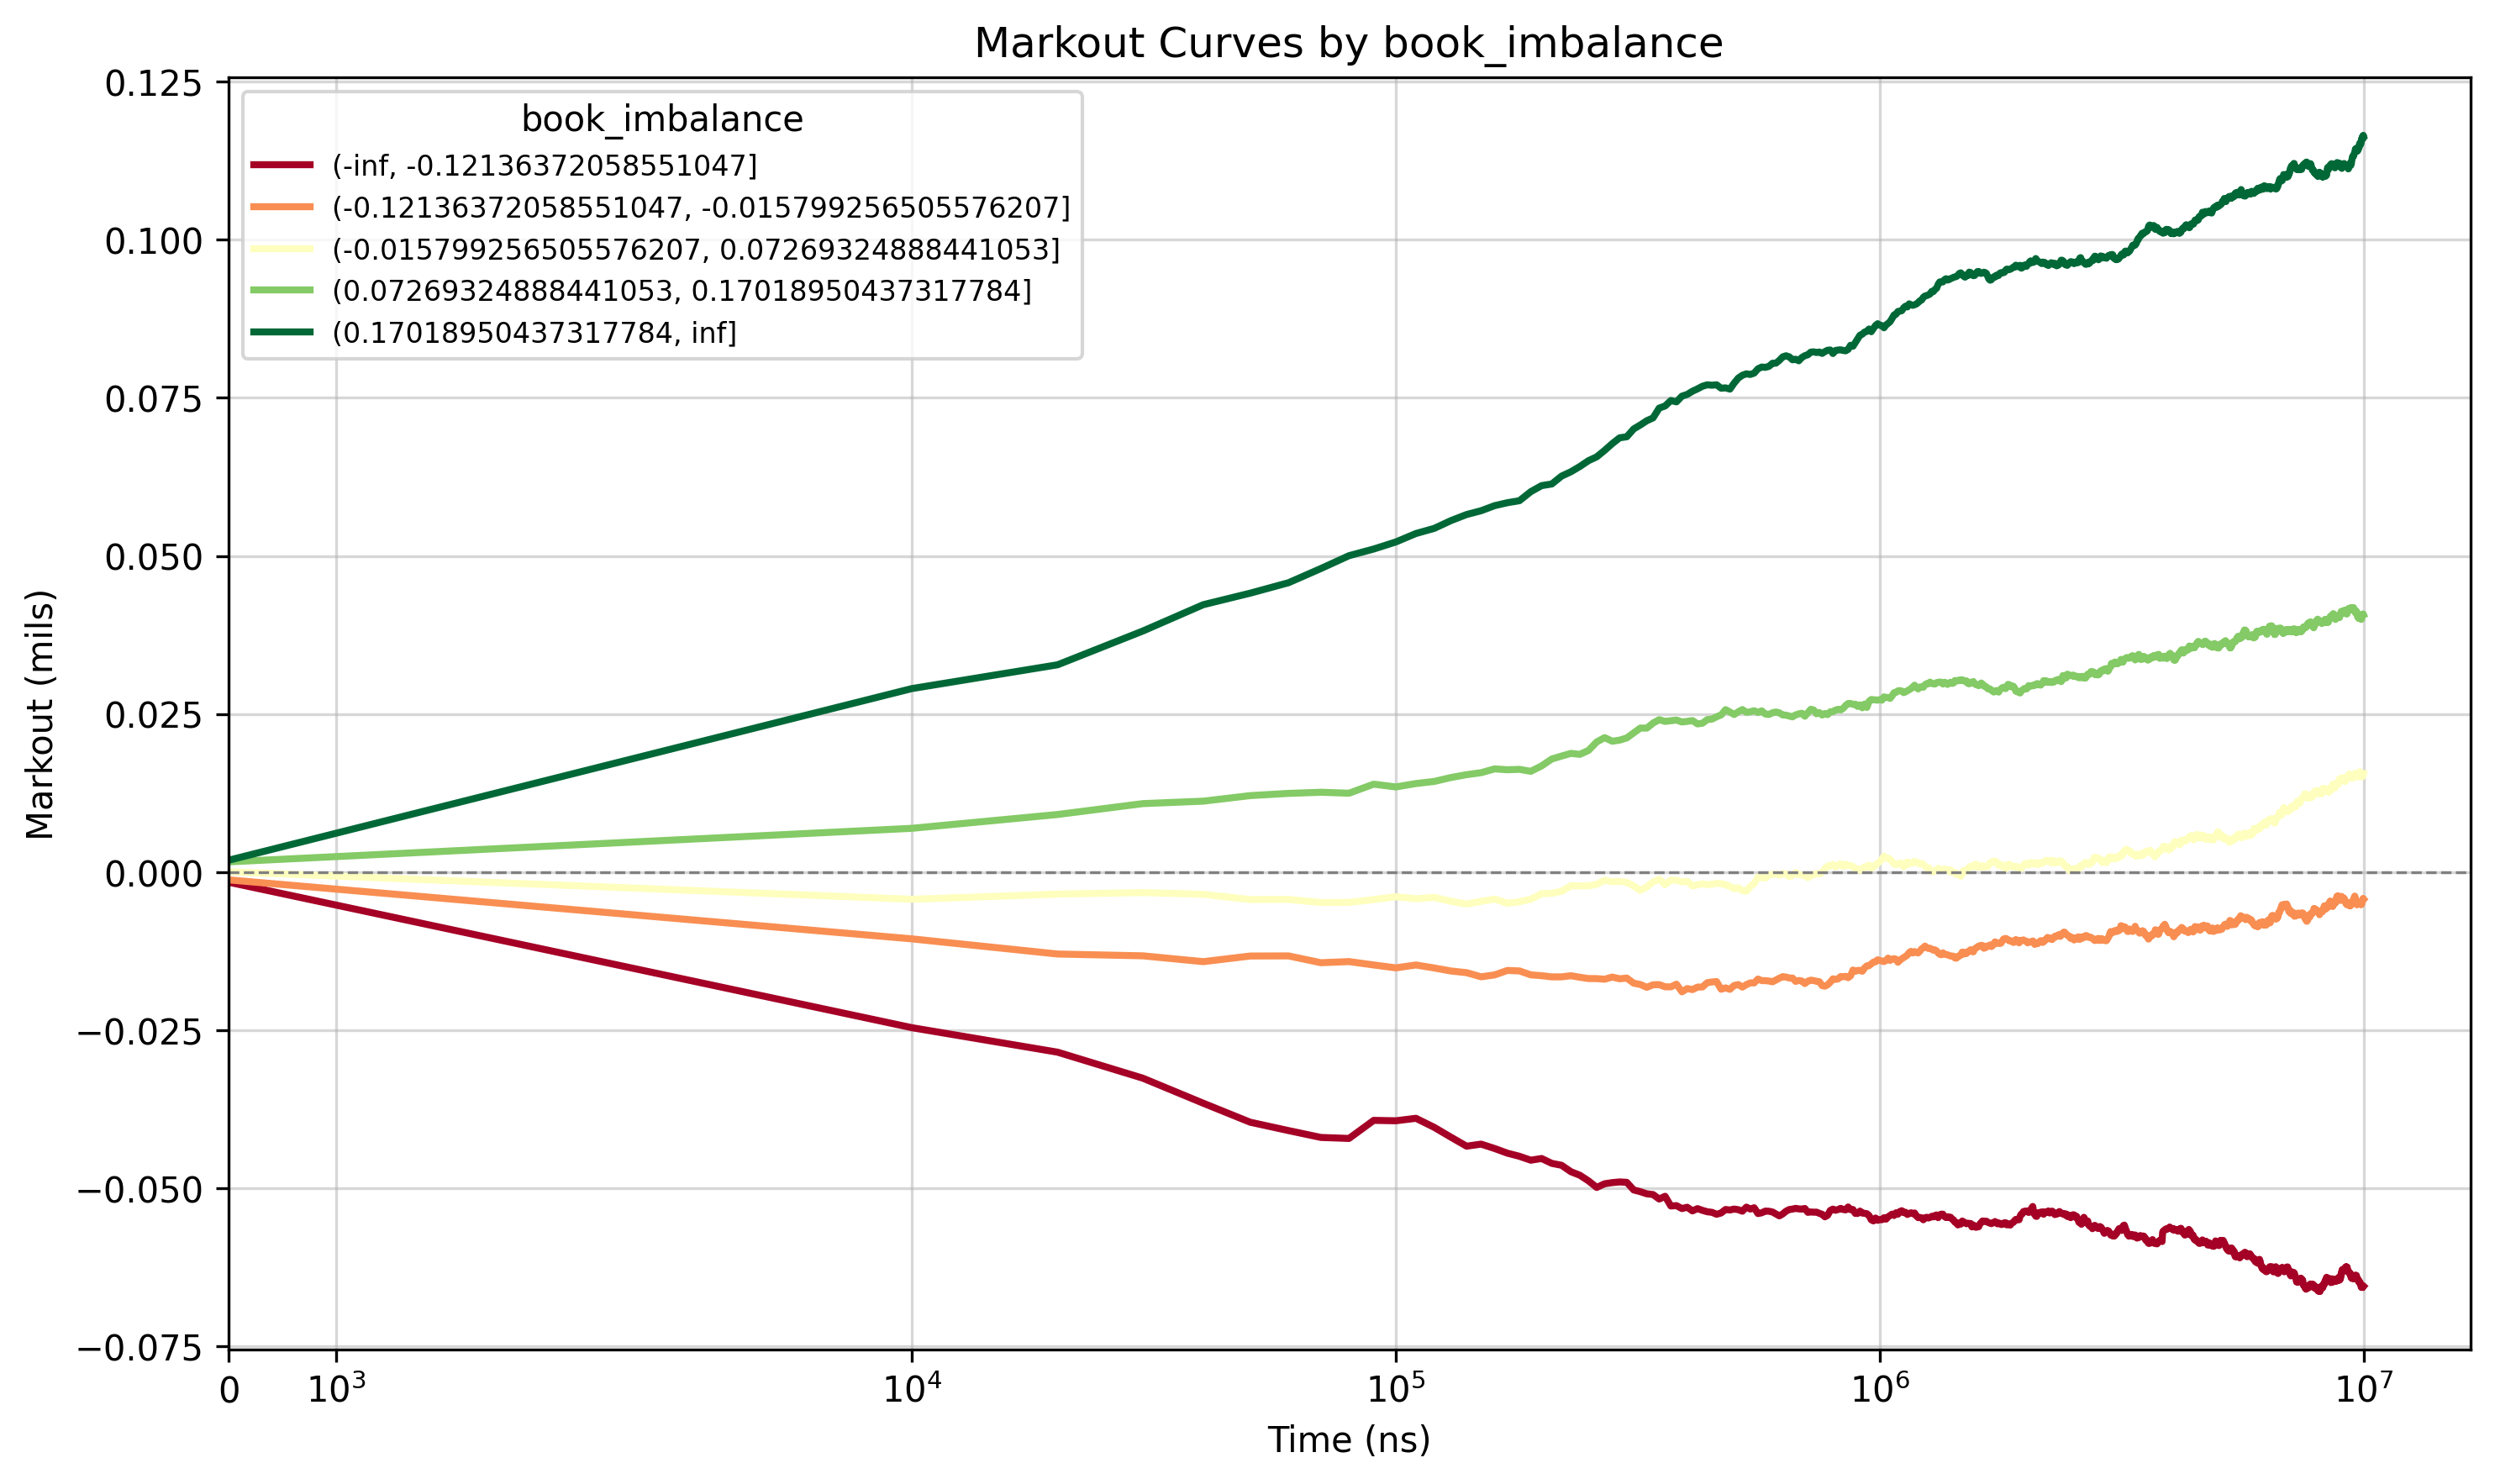
\includegraphics[keepaspectratio]{plots_and_data/section_1/markout_symlog.png}}

}

\caption{\label{fig-markout}Markout Plot}

\end{figure}%

\end{minipage}%

\end{figure}%

Figure~\ref{fig-markout} clearly shows that OBI is a powerful predictor
of price drift within milliseconds and that this price motion is
structural, indicated by the length of time that the markouts stay
smooth and near-zero variance. Using OBI's predictive qualities, our
fill strategy, discussed in Section~\ref{sec-hybrid} can reliably
predict positive and negative price drifts and only fill when
advantageous.

\section{Methodological Choices and
Innovations}\label{methodological-choices-and-innovations}

\subsection{Sourcing Data}\label{sourcing-data}

Throughout this work we utilize level 2 data in the \texttt{MBP-10}
schema from Databento, which provides the top 10 levels of the book for
a selection of stocks and dates. The dataset samples on all order book
updates (trades, adds, cancels, etc.) which allows us to reconstruct the
book over time. The data is sourced from
\href{https://databento.com/docs/schemas-and-data-formats/mbp-10?historical=python&live=python&reference=python}{Databento}.
We fetch data through a simple \texttt{DatabentoGenericAdapter} class
that uses a hierarchical caching structure. This allows us to call the
Databento API only for new data, which is necessary to manage time and
storage capacity for L2 book data. The adapter caches on
\texttt{{[}tickers,\ start,\ end,\ dataset,\ schema{]}}. Here, our
schema is always \texttt{MBP-10} and we use the \texttt{XNAS.ITCH}
Dataset which gives us full access to the Nasdaq exchange.

We use L2 data for three tickers, \texttt{AMZN}, \texttt{CSCO}, and
\texttt{DRH} from \texttt{"2026-03-18":"2026-04-18"}. We chose these
tickers because they are representative of three major varieties of
equities. \texttt{AMZN} is a liquid small-tick stock that should offer
ample resilience to price impact and relatively high and volatile
intraday bid-ask spreads. \texttt{CSCO} is a liquid large-tick stock
that still has deep liquidity but more narrow and consistent intraday
spreads. Finally, \texttt{DRH} is an illiquid large-tick stock that
offers a challenge to minimizing costs. It cannot accept large amounts
of liquidity, moves more slowly than \texttt{AMZN} and \texttt{CSCO}. It
also has more inconsistent order arrival rates, which poses a direct
challenge for using OBI as a signal. Altogether this dataset is 28.7GB,
on the order of RAM capacity for a sequential process but requires some
management for parallel processing tasks, like the below.

\subsection{Simulator}\label{sec-sim}

The technical backbone of this work is the \texttt{ExecutionSimulator}
class we designed to simulate fills using raw \texttt{MBP-10} data. The
simulator can do the following.

\begin{enumerate}
\def\labelenumi{\arabic{enumi}.}
\tightlist
\item
  Simulate the execution of market orders, resting limit orders, and
  immediate-or-cancel (IOC) limit orders at a given nanosecond timestamp
  and latency.
\item
  Maintain an orderbook state over time, using level two \texttt{MBP-10}
  data from Databento, consistent with mutations of the book caused by
  simulated fills and the replenishment of swept levels via a Poisson
  process with book-update sampling.
\item
  Calculate and track execution statistics (arrival cost, fill times,
  quantities, etc.) for any arbitrary execution strategy using the above
  order types.
\end{enumerate}

Our implementation of the \texttt{ExecutionSimulator} class initiates
the L2 book with a \texttt{polars} dataframe in Databento's
\texttt{MBP-10} schema. The simulator maintains the book using
internally consistent \texttt{numpy} arrays, which it updates as the
book mutates via simulated fills. After each simulated order is filled
(mainly child orders) the simulator returns a dictionary of the form
below. Note from Section~\ref{sec-definitions} that
\texttt{arrival\_cost} is calculated as the \texttt{vwap} minus the mid
price at execution. At the end of a simulation it returns a new
\texttt{polars} dataframe representing the mutated book over time
(sampled at book-update events) as well as a list of individual fill
results described in Section~\ref{sec-definitions}.

At each book update the simulator also replenishes any levels swept by
previous simulated fills. After each marketable order execution, the
simulator draws a limit order quantity \(q_i\) for each price tick
\(p_i\) between the best ask and best bid, using a Poisson distribution
at rate \(\lambda\) (set as a hyperparameter). If any \(q_i>0\), then a
limit order is added with quantity \(q_i\) at price level \(p_i\).

\subsection{Strategy Evaluation}\label{strategy-evaluation}

To evaluate each of the following strategies, we utilize a parallel
processing trial workflow. At initialization, we set the numerous
required hyperparameters, each listed below.

\begin{itemize}
\tightlist
\item
  \texttt{Latency}: 100us, \texttt{Poisson\ Replenishment}: 100.0,
  \texttt{PARENT\_QTY}: 10\_000, \texttt{MAX\_WORKERS}: 10,
  \texttt{N\_TRIALS}: 5\_000, \texttt{SEED}: 12345, \texttt{HORIZON}:
  300s
\end{itemize}

To load data while managing memory we scan the full dataset's cache and
split into one \texttt{.parquet} for each ticker. We then randomly
sample \texttt{N\_TRIALS} initial timestamps from the book, ensuring
that no two windows from the initial timestamp through the
\texttt{HORIZON} overlap more than a few seconds. Then for each
combination of asset and fill strategy, we initialize
\texttt{MAX\_WORKERS} CPU workers and scan the relevant ticker
\texttt{.parquet} file for each window and run the fill strategy on that
window only, randomly sampling the side of the order from
\texttt{{[}\textquotesingle{}BUY\textquotesingle{},\ \textquotesingle{}SELL\textquotesingle{}{]}}.
This workflow balances memory requirements and parallelized processing
speed. Compared with the sequential workflow used in the milestone
report, this brought down the time cost from half an hour per trial over
the full dataset to a few seconds per trial over a selected window.

To measure the performance of each fill strategy, we save information
including \texttt{side}, \texttt{parent\_filled},
\texttt{parent\_arrival\_cost}, \texttt{mean\_child\_arrival\_cost},
\texttt{median\_child\_arrival\_cost}, and \texttt{parent\_lifetime}.
Below we compare our final successful strategy with the naive strategy
using the above metrics, and go over some failed innovations and their
associated learnings along the way. More on specific definitions of the
above metrics can be found in Section~\ref{sec-definitions}.

\subsection{Naive Benchmark}\label{naive-benchmark}

As discussed and plotted earlier, we are comparing our strategies with
the naive method of splitting orders into \texttt{N\_CHUNKS\ =\ 50}, and
filling them a fixed time interval \texttt{WAIT\_TIME\ =\ 1s} apart
using regular market orders. Table~\ref{tbl-naive} shows some
performance metrics for this naive method filling ten-thousand shares of
\texttt{CSCO} to serve as a benchmark we are competing against.

\begin{longtable}[]{@{}llllll@{}}

\caption{\label{tbl-naive}Naive Results}

\tabularnewline

\toprule\noalign{}
statistic & total\_filled & parent\_cost & mean\_child\_cost &
median\_child\_arrival\_cost & lifetime\_s \\
str & f64 & f64 & f64 & f64 & f64 \\
\midrule\noalign{}
\endhead
\bottomrule\noalign{}
\endlastfoot
"mean" & 10000.0 & 9.8626 & 5.798219 & 4.182775 & 9.582253 \\
"min" & 10000.0 & -21.535187 & 1.374581 & 0.580619 & 6.221948 \\
"25\%" & 10000.0 & 6.428417 & 3.883612 & 3.316627 & 9.524487 \\
"50\%" & 10000.0 & 9.053304 & 5.149228 & 3.90504 & 9.687721 \\
"75\%" & 10000.0 & 12.472484 & 7.069212 & 4.637834 & 9.761385 \\
"max" & 10000.0 & 61.71924 & 36.425326 & 35.814917 & 9.800094 \\

\end{longtable}

\subsection{Failure: Naive with IOC}\label{failure-naive-with-ioc}

The first pass attempt to improve on the benchmark is simply running the
same strategy using marketable IOC limit orders instead of market
orders. Results below in Table~\ref{tbl-naive-ioc}. We set the limit
price of each child order to the 10th level of the ask (bid) for a
parent buy (sell) order at the initial time of execution. This resulted
in better fills, however it almost never completed the full parent order
given its simple cap on the allowed execution price.

\begin{longtable}[]{@{}llllll@{}}

\caption{\label{tbl-naive-ioc}Naive IOC Results}

\tabularnewline

\toprule\noalign{}
statistic & total\_filled & parent\_cost & mean\_child\_cost &
median\_child\_arrival\_cost & lifetime\_s \\
str & f64 & f64 & f64 & f64 & f64 \\
\midrule\noalign{}
\endhead
\bottomrule\noalign{}
\endlastfoot
"mean" & 7818.5352 & 5.28774 & 3.374856 & 3.293796 & 8.880517 \\
"min" & 200.0 & -21.525161 & 1.207293 & 0.580619 & 0.0 \\
"25\%" & 6838.0 & 4.482656 & 3.052005 & 2.950195 & 8.446878 \\
"50\%" & 7905.0 & 5.518874 & 3.353437 & 3.200819 & 9.370963 \\
"75\%" & 8967.0 & 6.410203 & 3.658963 & 3.726398 & 9.709241 \\
"max" & 10000.0 & 29.237672 & 16.116962 & 15.40023 & 9.800094 \\

\end{longtable}

\subsection{Failure: OBI Aggressive
Only}\label{failure-obi-aggressive-only}

Beyond simply tweaking the benchmark our first true pass at an
improvement used OBI to time our fills using the parameter
\texttt{OBI\_THRESHOLD\ =\ 0.85}. First, set the maximum size of a child
fill at \(q_{max}\). For a buy order, if the OBI was above the threshold
that indicated an expected upward price move, the logic is to fill a
child order immediately of size \(q_{max} * |OBI|\), where
\(q_{max} = 350\). This would dynamically size orders based on the size
of the subsequent price moves, and attempt to only fill at advantageous
times. Figure~\ref{fig-obi} shows this strategy in action.

\begin{figure}

\centering{

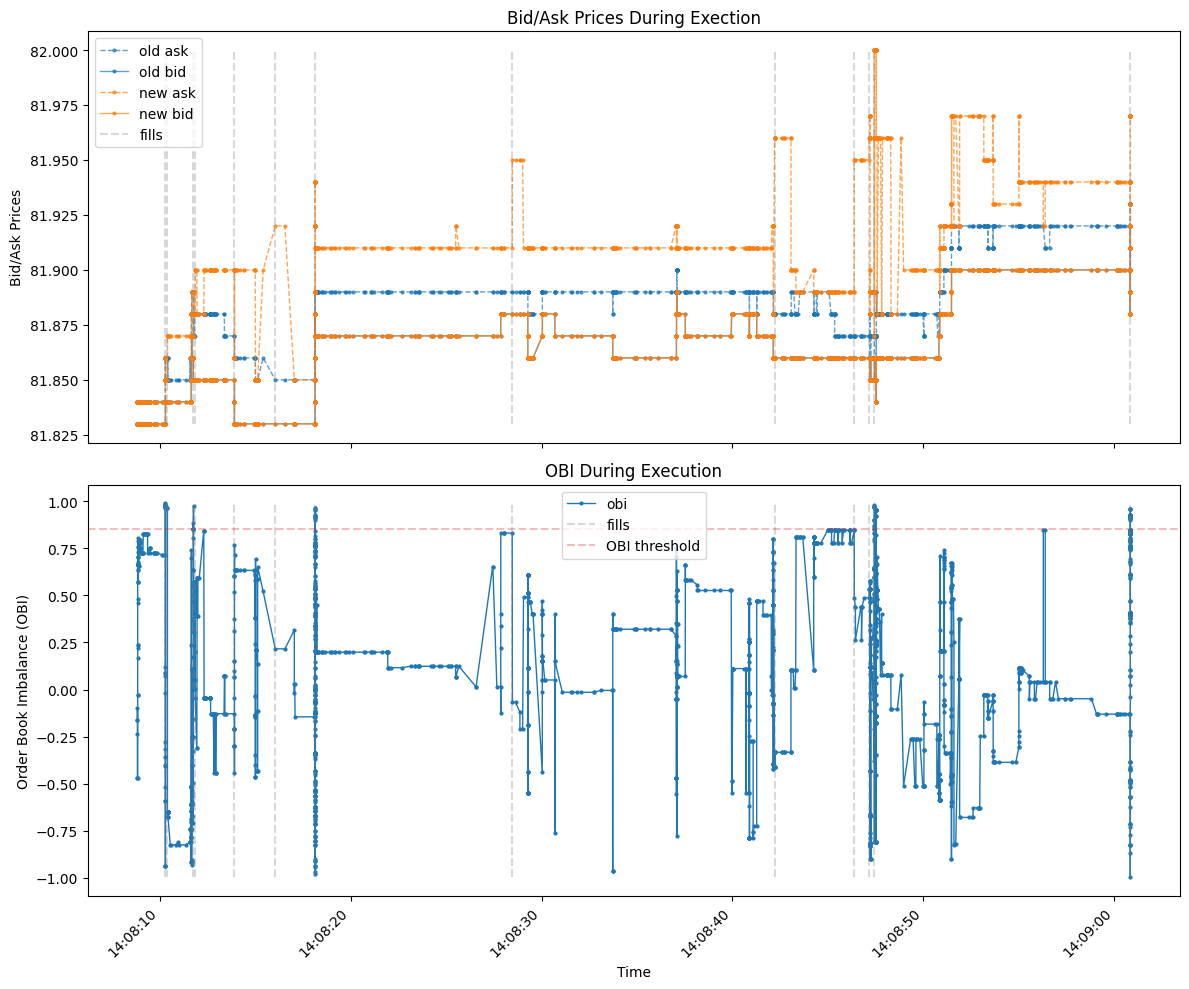
\includegraphics[width=0.8\linewidth,height=\textheight,keepaspectratio]{plots_and_data/section_2/failed_runs/obi_aggressive.png}

}

\caption{\label{fig-obi}OBI Aggressive Only Fills}

\end{figure}%

This strategy has a few issues. Firstly, for some time horizons, OBI
infrequently or simply never hits the threshold and so the parent order
only gets a partial fill. More fundamentally, this logic only seeks to
avoid adverse fill conditions, and does nothing explicit to take
advantage of favorable ones.

The aggressive-only OBI logic originated from a way of thinking rooted
in alpha generation and the predicted returns to be exploited by taking
an aggressive position. But returns are exactly \emph{not} what an
execution strategy is focused on: simply put, to take advantage of alpha
a strategy must enter and exit a position, but an execution strategy is
\emph{given} a predetermined order to place and its task is to minimize
the cost filling the order's quantity over a set time horizon. Solving
the second issue via this change of perspective lead directly to our
improvement via a hybrid strategy.

\subsection{Final Strategy: Imbalance Calibrated
Aggression}\label{sec-hybrid}

After escaping the alpha generation line of thinking, we were able to
develop a much more effective fill strategy. It is a hybrid of the naive
and OBI strategies that uses OBI to calibrate the aggressiveness or
urgency of fills. For a parent order of quantity \(q\) logic is as
follows:

\begin{enumerate}
\def\labelenumi{\arabic{enumi}.}
\tightlist
\item
  Split the parent order into \(n\) child orders of size \(q/n\).
\item
  Set positive and negative OBI thresholds for expected price moves that
  are calibrated using the markout plots above.
\item
  For a buy order, depending on the value of OBI, do the following (or
  opposite for a sell):
\end{enumerate}

\begin{itemize}
\tightlist
\item
  If OBI \textgreater{} \texttt{OBI\_THRESHOLD}, expect an adverse price
  move. Fill one child order immediately. Cross the spread with an IOC
  limit order and limit price set to the 10th level of the book at the
  time the parent order was split.
\item
  If OBI \textless{} -1 * \texttt{OBI\_THRESHOLD}, expect a favorable
  price move. Place resting limit orders at each of the top ten bids,
  each for the quantity of one child order. Set expiry at the end of the
  parent order's allowed horizon.
\item
  If OBI is between the above thresholds, fill child orders with IOC
  limit orders at a slow constant rate with the same limit price.
\end{itemize}

By calibrating the aggression of child orders and allowing the price to
drift, this strategy fills the vast majority of shares during favorable
price conditions, and avoids unfavorable ones by filling immediately and
then not at all until the price moves favorably again. This is
illustrated in Figure~\ref{fig-hybrid}, which shows the true and
simulated best bid and ask over time with favorable and adverse price
drifts highlighted using the value of OBI. The vertical gray markers are
the timestamps of each child fill. Note that limit orders placed when
OBI is low may fill when OBI is high, resulting in lots of fills during
times marked ``unfavorable''. This is positive and expected behavior.

\begin{figure}

\centering{

\pandocbounded{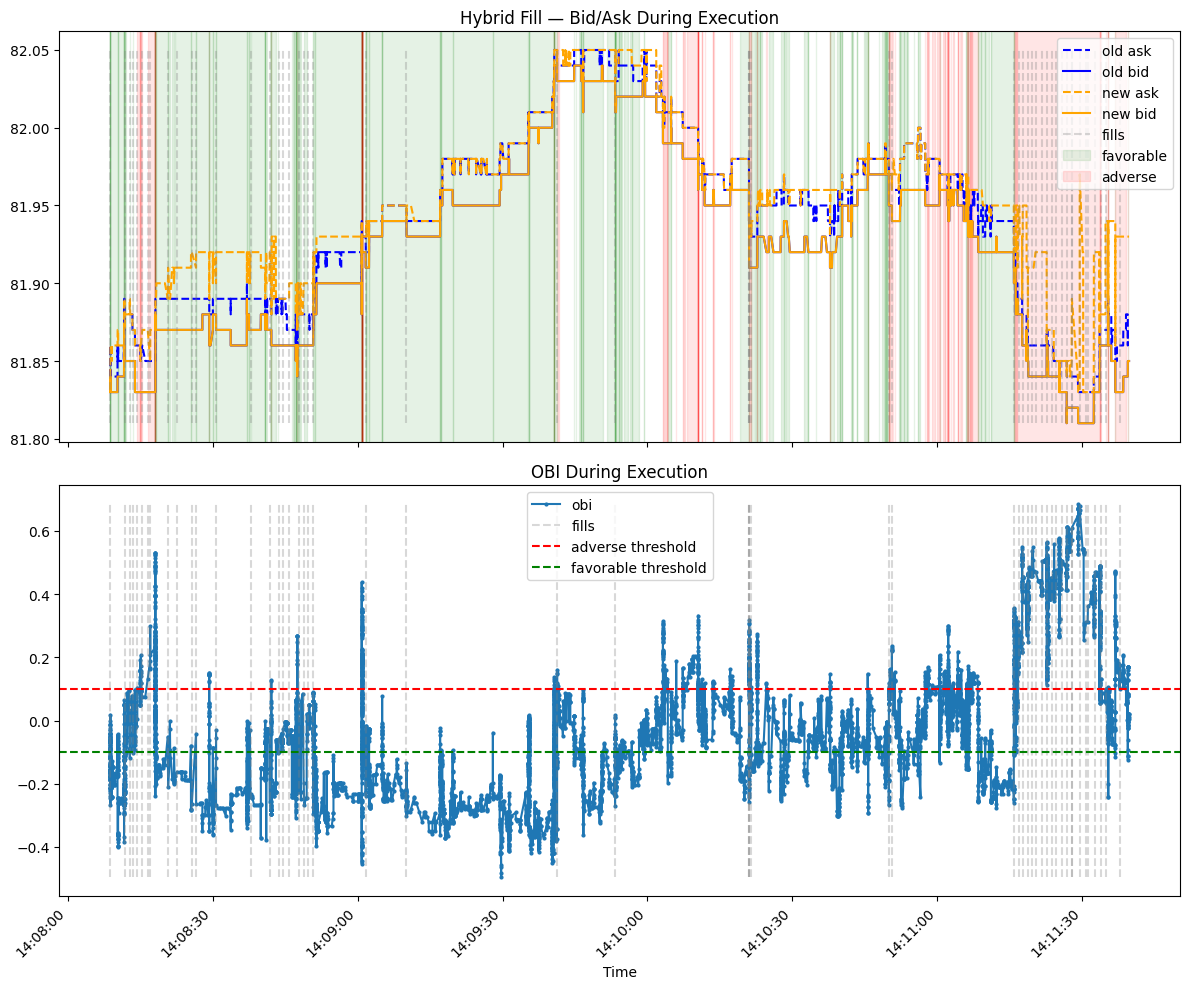
\includegraphics[keepaspectratio]{plots_and_data/section_3/successful_run/hybrid.png}}

}

\caption{\label{fig-hybrid}Hybrid Fill Strategy}

\end{figure}%

\section{Empirical Findings}\label{empirical-findings}

Table~\ref{tbl-success} shows some descriptive statistics of the results
of the hybrid fill strategy, by asset, and Table~\ref{tbl-tstat} in
Section~\ref{sec-tstat} shows the means of the naive and hybrid
strategies alongside their statistical significance demonstrated by a
t-test. Parent costs are measured in bps per share. These results are
derived from running the strategy across assets for 5000 timestamps,
latency of \texttt{100us}, replenishment rate of \(\lambda = 15\) (which
is quite low), a time horizon of \(5\) minutes, and splitting a 10,000
share parent order into \(n=50\) child orders each with quantity
\(q=200\) with OBI thresholds of \(\pm 0.10\).

The average parent order's total cost, defined in
Section~\ref{sec-definitions}, is highly dependent on the liquidity of
each stock, with \texttt{DRH} and \texttt{CSCO} fills being respectively
141x and 9x times more costly than \texttt{AMZN} on average. This is
likely the result of illiquidity causing child orders to have higher
mechanical price impact, and methods to improve this are considered in
Section~\ref{sec-future}. The order lifetimes are relatively consistent
at approximately thirty seconds for the liquid stocks, and above a
minute for illiquid. All hybrid fills were completed within the 5 minute
horizon. Figure~\ref{fig-hist} shows histograms of the total parent cost
per asset. Here it is visually obvious that the naive method has a heavy
right tail, while the hybrid strategy has a mean shift downward and
heavy left tail. Its ability to deliver these results with such a low
replenishment rate simulating small sub-100-share limit order
replenishment is impressive.

\begin{figure}

\begin{minipage}{0.33\linewidth}

\centering{

\pandocbounded{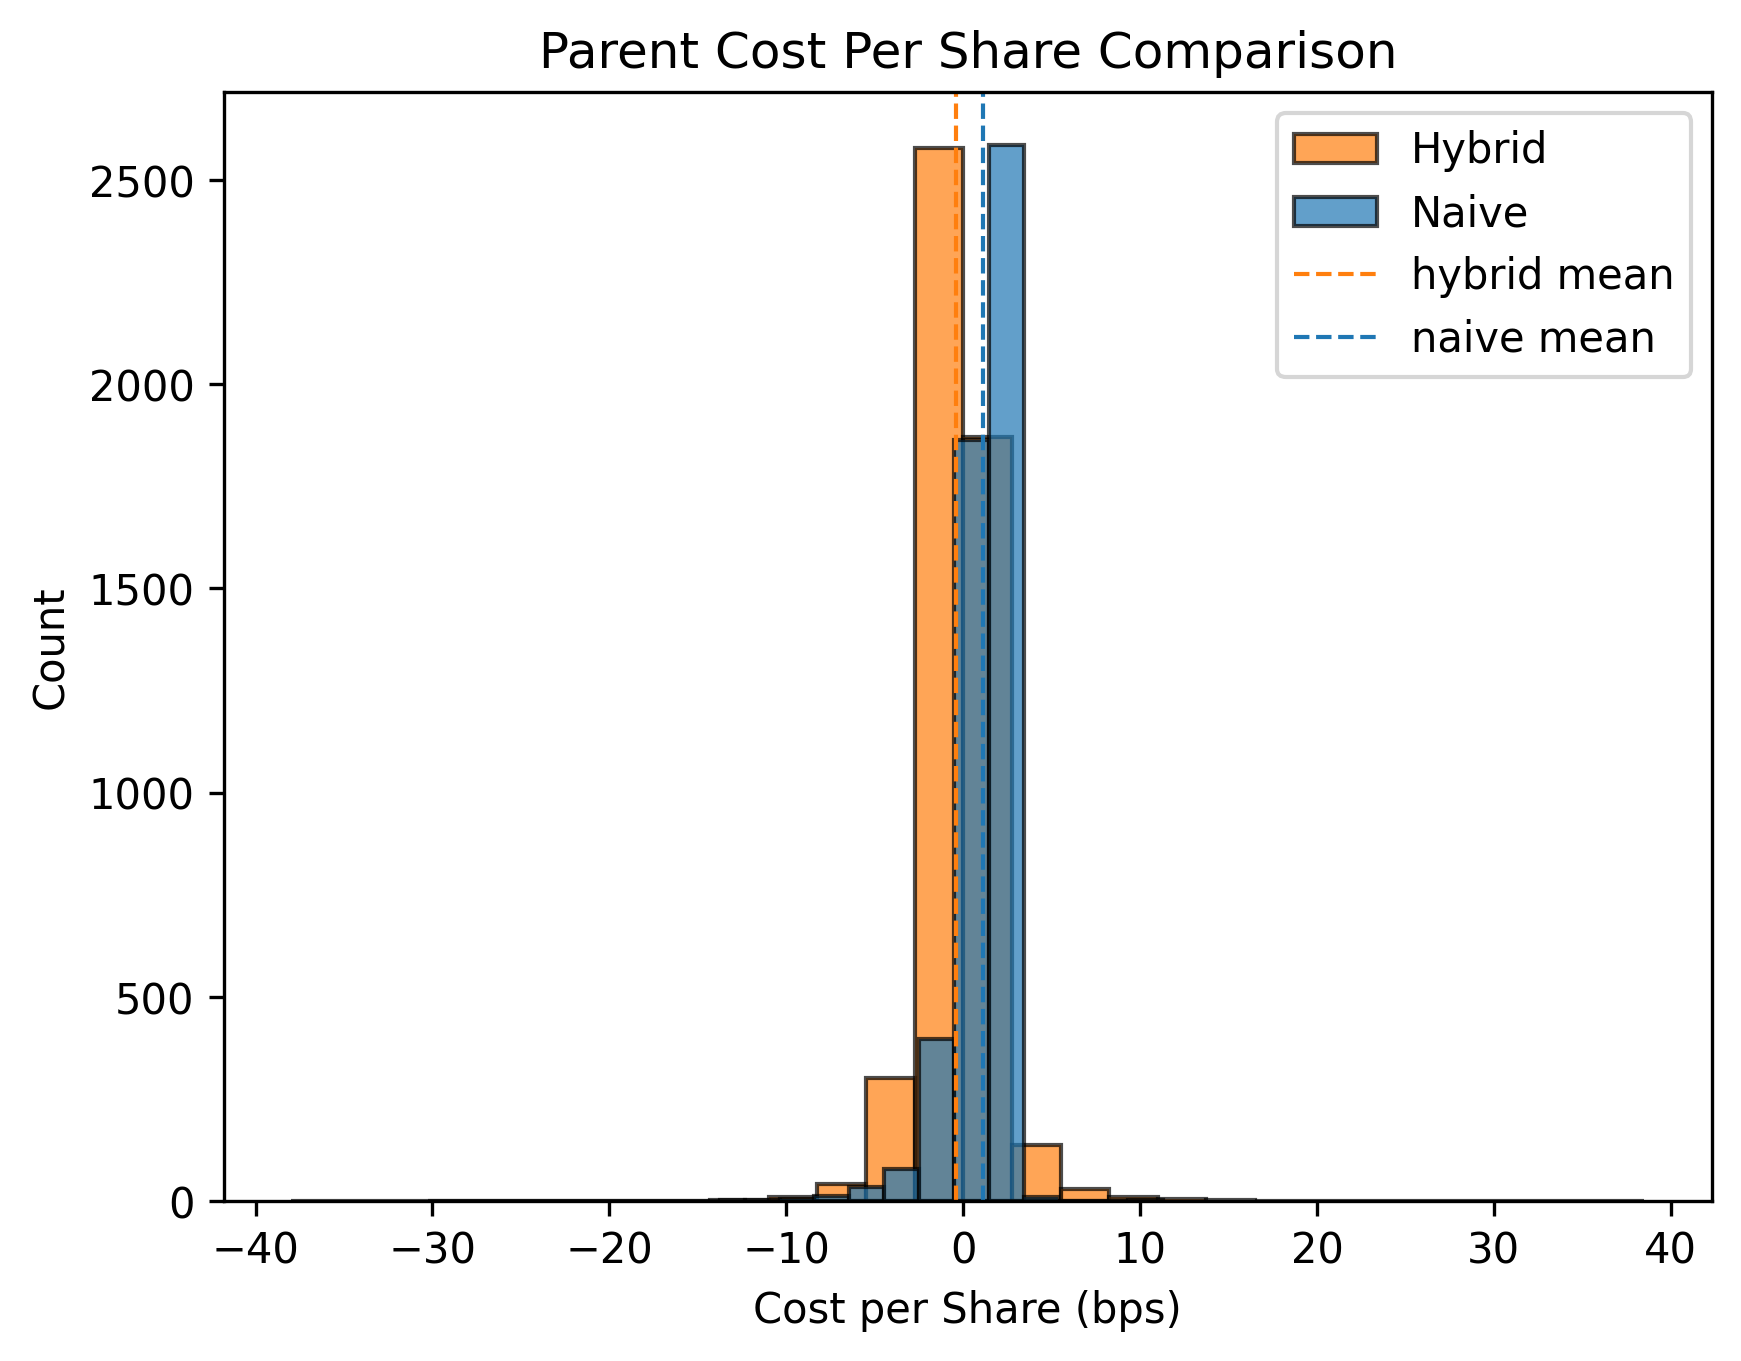
\includegraphics[keepaspectratio]{plots_and_data/section_3/successful_run/plots/parent_cost_mid.AMZN.png}}

}

\subcaption{\label{fig-hybrid}AMZN}

\end{minipage}%
%
\begin{minipage}{0.33\linewidth}

\centering{

\pandocbounded{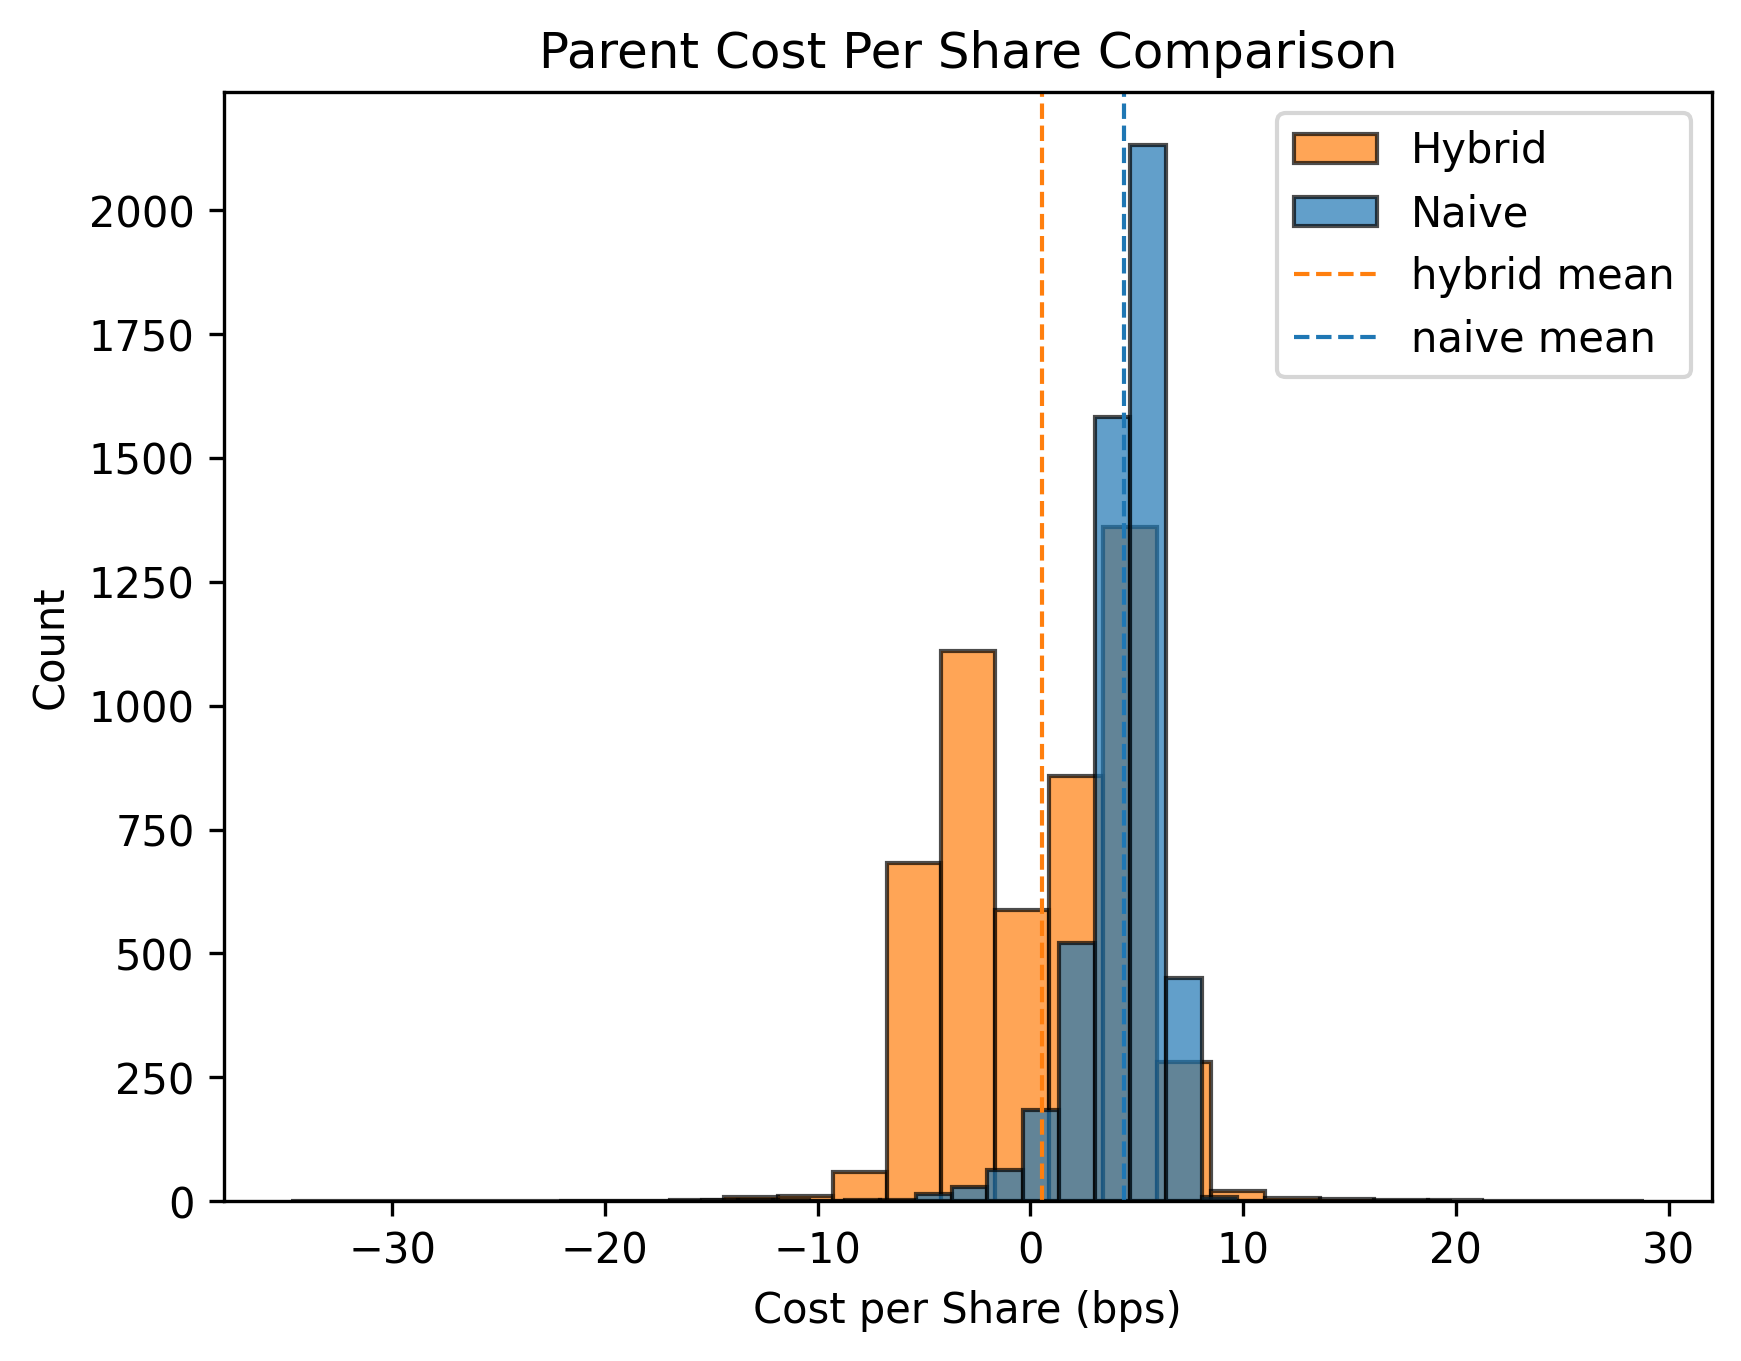
\includegraphics[keepaspectratio]{plots_and_data/section_3/successful_run/plots/parent_cost_mid.CSCO.png}}

}

\subcaption{\label{fig-hybrid}CSCO}

\end{minipage}%
%
\begin{minipage}{0.33\linewidth}

\centering{

\pandocbounded{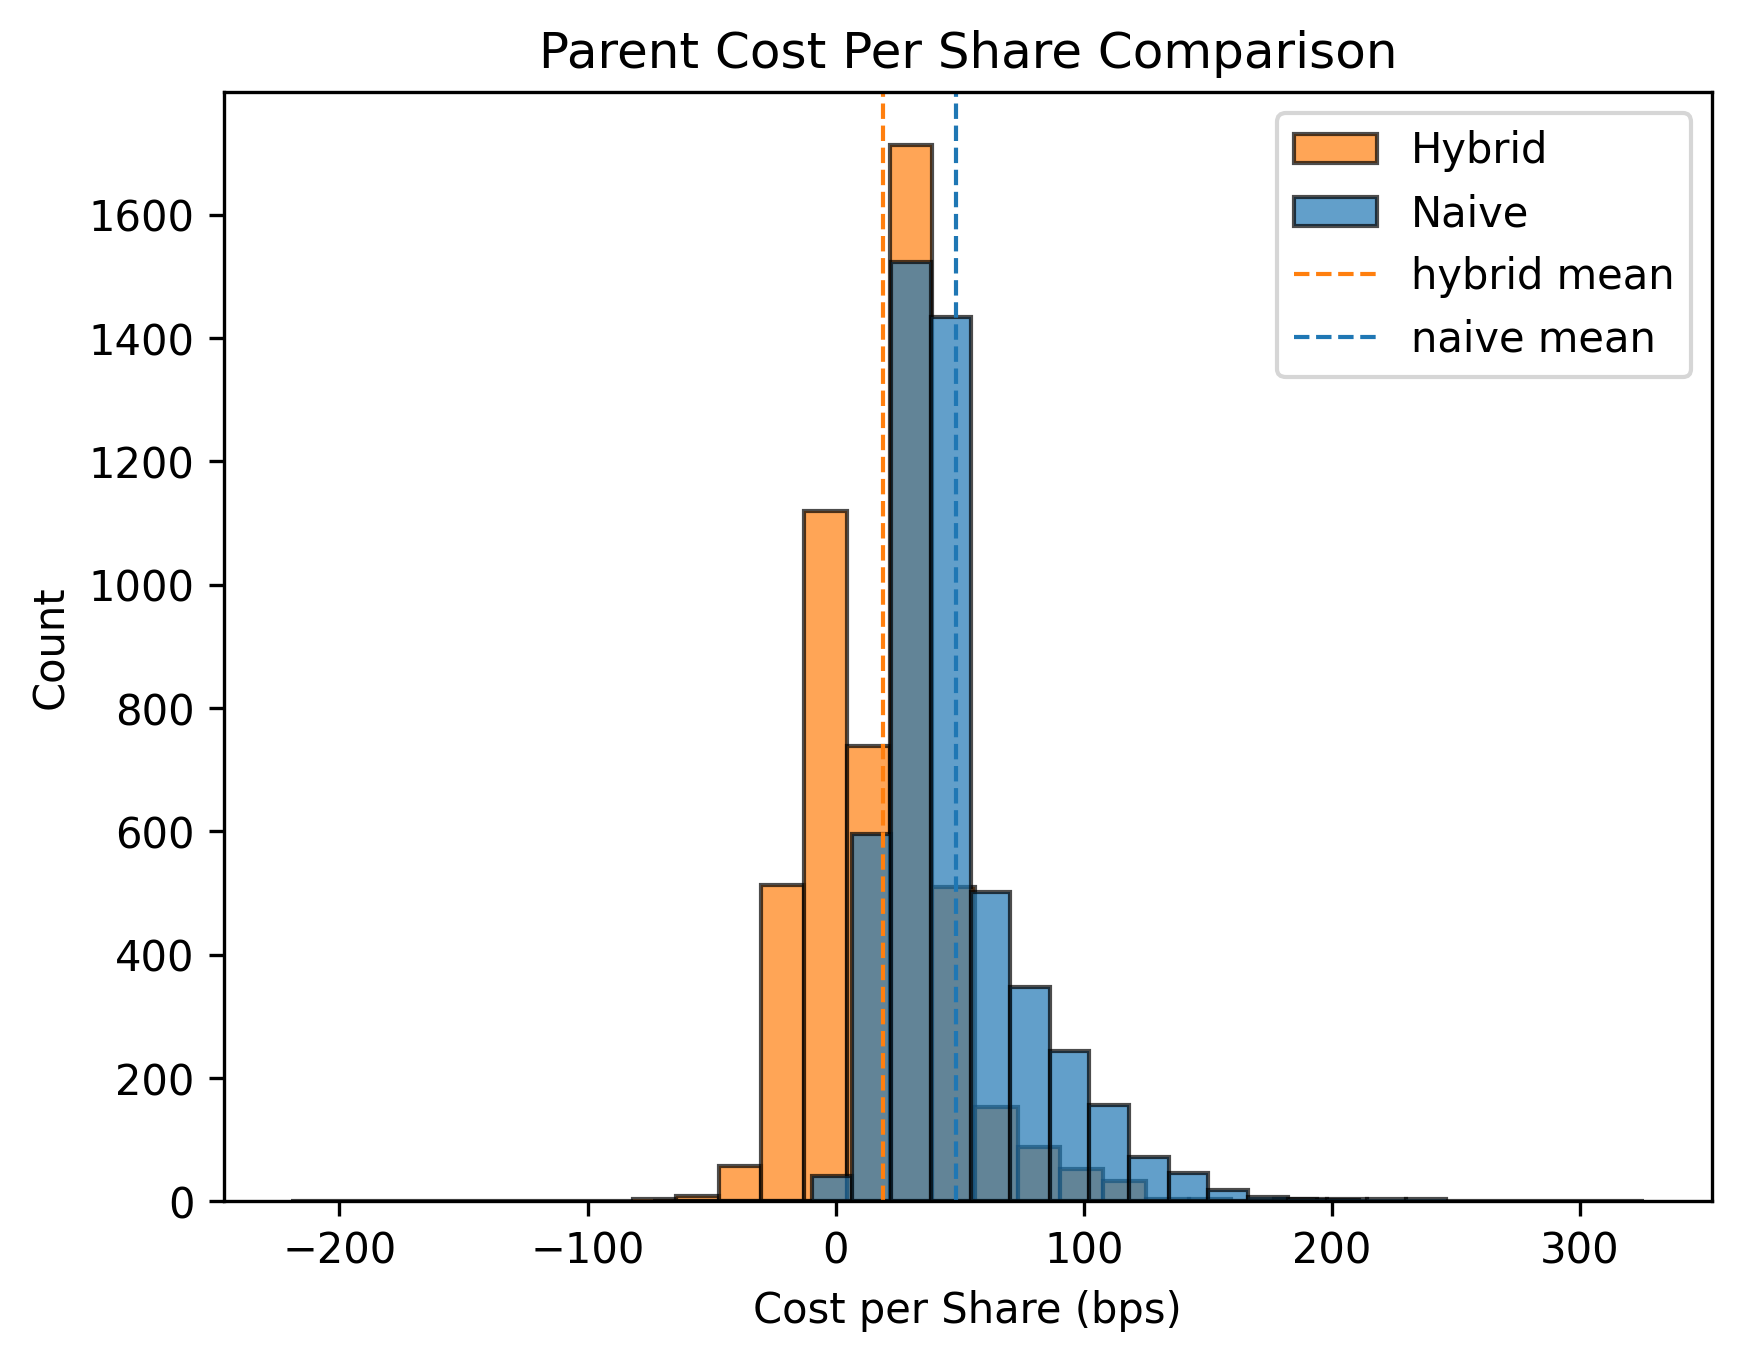
\includegraphics[keepaspectratio]{plots_and_data/section_3/successful_run/plots/parent_cost_mid.DRH.png}}

}

\subcaption{\label{fig-hybrid}DRH}

\end{minipage}%

\caption{\label{fig-hist}Total Parent Cost Comparison}

\end{figure}%

\begin{table}

\caption{\label{tbl-success}Hybrid Fill Statistics}

\begin{minipage}{0.47\linewidth}

\subcaption{\label{tbl-success-1}AMZN}

\centering{

\begin{tabular}{lll}
\toprule
statistic & parent\_cost & lifetime\_s\\
\midrule
str & f64 & f64\\
"mean" & 0.184687 & 28.482708\\
"std" & 2.185917 & 45.185725\\
"50\%" & 0.069449 & 13.0227\\
\bottomrule
\end{tabular}

}

\end{minipage}%
%
\begin{minipage}{0.05\linewidth}
~\end{minipage}%
%
\begin{minipage}{0.47\linewidth}

\subcaption{\label{tbl-success-2}CSCO}

\centering{

\begin{tabular}{lll}
\toprule
statistic & parent\_cost & lifetime\_s\\
\midrule
str & f64 & f64\\
"mean" & 1.496204 & 32.403243\\
"std" & 4.217447 & 49.10376\\
"50\%" & 2.133194 & 15.597951\\
\bottomrule
\end{tabular}

}

\end{minipage}%
\newline
\begin{minipage}{\linewidth}

\subcaption{\label{tbl-success-3}DRH}

\centering{

\begin{tabular}{lll}
\toprule
statistic & parent\_cost & lifetime\_s\\
\midrule
str & f64 & f64\\
"mean" & 25.47164 & 75.61788\\
"std" & 28.592753 & 92.533696\\
"50\%" & 28.342588 & 31.240362\\
\bottomrule
\end{tabular}

}

\end{minipage}%

\end{table}%

\subsection{Test Stats / Significance}\label{sec-tstat}

Table~\ref{tbl-tstat} shows the average cost in bps per share, per
ticker, using the hybrid and naive fill strategies, as well as the
results of a paired T-test sampled per asset. The hybrid strategy shows
a pronounced downward shift in cost across assets, with improvements of
89\% for \texttt{AMZN}, 73\% for \texttt{CSCO}, and 55\% for
\texttt{DRH}. Each of these results is also highly significant. We chose
to use a paired t-test since each strategy was run on the same 5,000
time windows, and therefore an independent t-test would be the wrong
choice.

\begin{longtable}[]{@{}lllll@{}}

\caption{\label{tbl-tstat}Paired T-Test on Arrival Cost per Asset}

\tabularnewline

\toprule\noalign{}
symbol & hybrid mean & naive mean & t\_stat & p\_val \\
str & f64 & f64 & f64 & f64 \\
\midrule\noalign{}
\endhead
\bottomrule\noalign{}
\endlastfoot
"AMZN" & 0.18 & 1.59 & 33.74 & 0.0 \\
"CSCO" & 1.5 & 5.24 & 56.09 & 0.0 \\
"DRH" & 25.47 & 54.43 & 50.81 & 0.0 \\

\end{longtable}

\subsection{Effects of Latency and
Replenishment}\label{effects-of-latency-and-replenishment}

In Table~\ref{tbl-latency} and Table~\ref{tbl-replenishment} we
demonstrate the hybrid strategy's robustness to latency and
replenishment. Here, latency is implemented as a delay between the time
each child order is sent and when it enters the book, and is displayed
in microseconds. The bps per-share cost differences between levels of
latency are remarkably low across assets and strategies. This is obvious
for the naive strategy as it is zero-intelligence. The hybrid strategy
does have some reliance on latency when filling with an IOC order
immediately before adverse moves, however the majority of fills are from
resting limit orders filling over multiple seconds and so it remains
robust to changes in latency, even up to fifty milliseconds.

The effects of low replenishment are also small but are more clear than
latency, while both strategies benefit heavily from a high rate of
replenishment. Across strategy and asset, a higher rate \(\lambda=200\)
leads to a lower price impact and thus lower average costs. This is
simply calibration of the book's liquidity, and demonstrates a sanity
check on the fill results.

\begin{longtable}[]{@{}lllll@{}}

\caption{\label{tbl-latency}Effects of Latency}

\tabularnewline

\toprule\noalign{}
symbol & latency\_level & hybrid mean cost & naive mean cost & latency
(us) \\
str & str & f64 & f64 & f64 \\
\midrule\noalign{}
\endhead
\bottomrule\noalign{}
\endlastfoot
"CSCO" & "low" & 4.19 & 9.76 & 10.0 \\
"AMZN" & "low" & 1.36 & 4.3 & 10.0 \\
"DRH" & "low" & 35.53 & 88.32 & 10.0 \\
"CSCO" & "mid" & 4.19 & 9.86 & 100.0 \\
"AMZN" & "mid" & 1.42 & 4.17 & 100.0 \\
"DRH" & "mid" & 35.62 & 88.36 & 100.0 \\
"CSCO" & "high" & 4.38 & 10.27 & 50000.0 \\
"AMZN" & "high" & 1.35 & 4.37 & 50000.0 \\
"DRH" & "high" & 35.64 & 88.54 & 50000.0 \\

\end{longtable}

\begin{longtable}[]{@{}lllll@{}}

\caption{\label{tbl-replenishment}Effects of Replenishment}

\tabularnewline

\toprule\noalign{}
symbol & replenishment\_level & hybrid mean cost & naive mean cost &
replenishment \\
str & str & f64 & f64 & f64 \\
\midrule\noalign{}
\endhead
\bottomrule\noalign{}
\endlastfoot
"CSCO" & "low" & 5.37 & 13.63 & 1.0 \\
"AMZN" & "low" & 2.03 & 6.9 & 1.0 \\
"DRH" & "low" & 42.01 & 94.8 & 1.0 \\
"CSCO" & "mid" & 4.19 & 9.86 & 15.0 \\
"AMZN" & "mid" & 1.42 & 4.17 & 15.0 \\
"DRH" & "mid" & 35.62 & 88.36 & 15.0 \\
"CSCO" & "high" & -1.51 & 2.62 & 200.0 \\
"AMZN" & "high" & -1.38 & 0.38 & 200.0 \\
"DRH" & "high" & 14.48 & 38.46 & 200.0 \\

\end{longtable}

\subsection{Intraday Seasonality}\label{intraday-seasonality}

Figure~\ref{fig-time} shows the intraday seasonality of median arrival
cost in bps per-share, across tickers and strategies. As expected both
strategies, though especially the hybrid, benefit from the high volume
on the open, and approach a mean throughout the day. Interestingly, the
naive strategy does worst at the open for DRH. This is likely a result
of both high opening spreads and low top book depth on open for the
illiquid asset, which then stabilize over time. This effect is
demonstrated in
\href{https://saf.jeremyshen.com/notes/lecture/lec8.html\#basic-trading-slangs}{Lecture
8}.

\begin{figure}

\begin{minipage}{0.50\linewidth}

\centering{

\pandocbounded{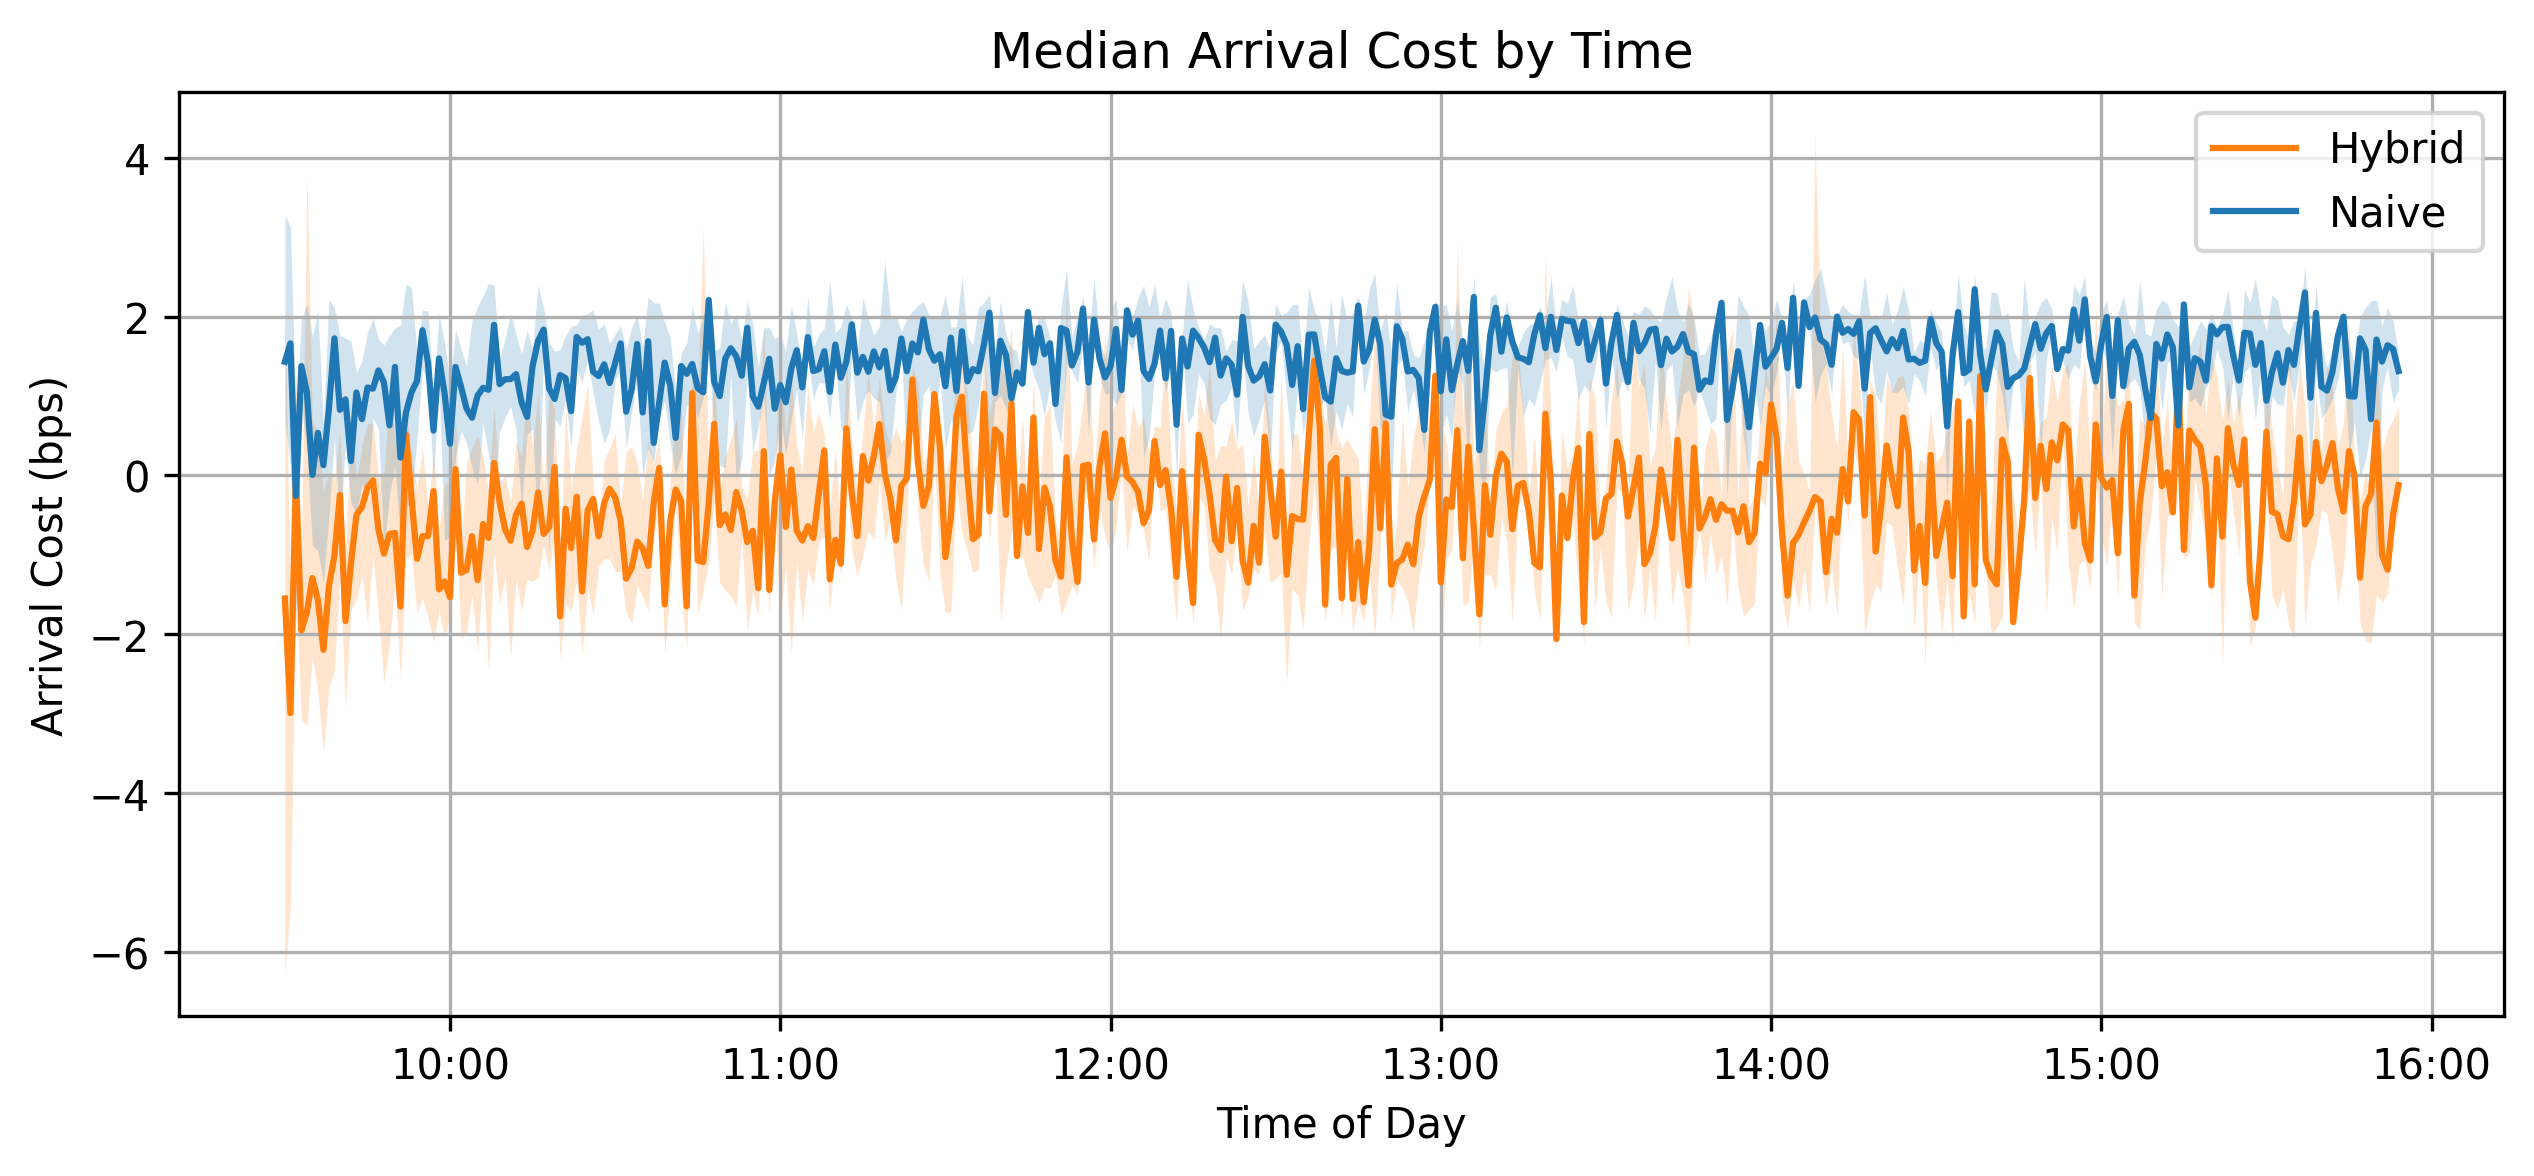
\includegraphics[keepaspectratio]{plots_and_data/section_3/successful_run/plots/time_mid.AMZN.png}}

}

\subcaption{\label{fig-time-amzn}AMZN}

\end{minipage}%
%
\begin{minipage}{0.50\linewidth}

\centering{

\pandocbounded{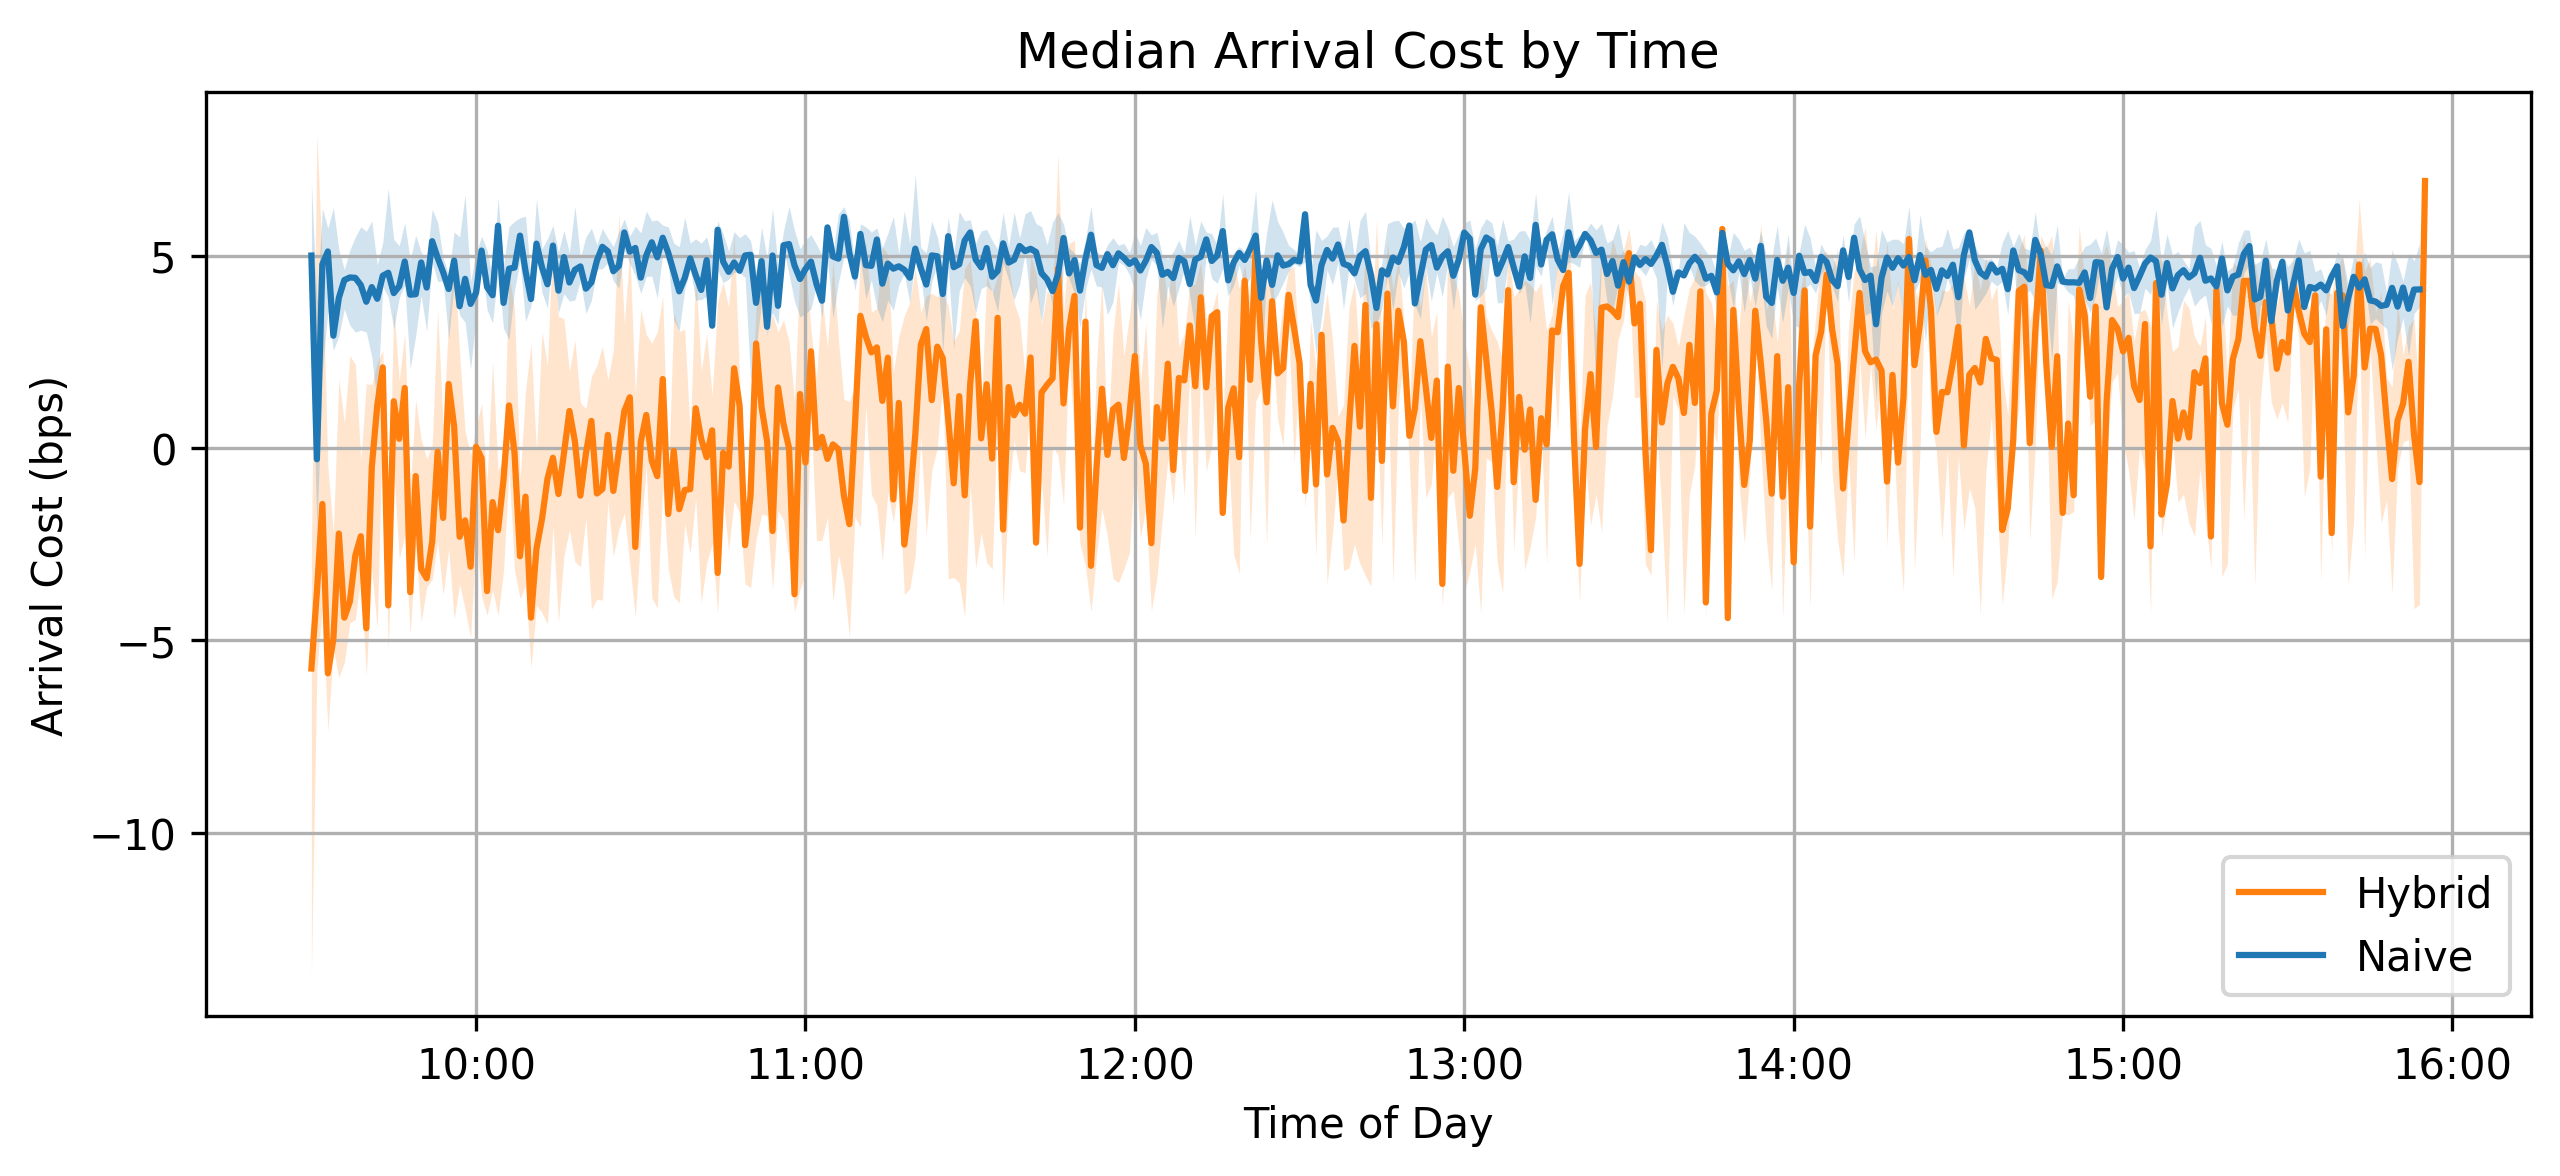
\includegraphics[keepaspectratio]{plots_and_data/section_3/successful_run/plots/time_mid.CSCO.png}}

}

\subcaption{\label{fig-time-csco}CSCO}

\end{minipage}%
\newline
\begin{minipage}{\linewidth}

\centering{

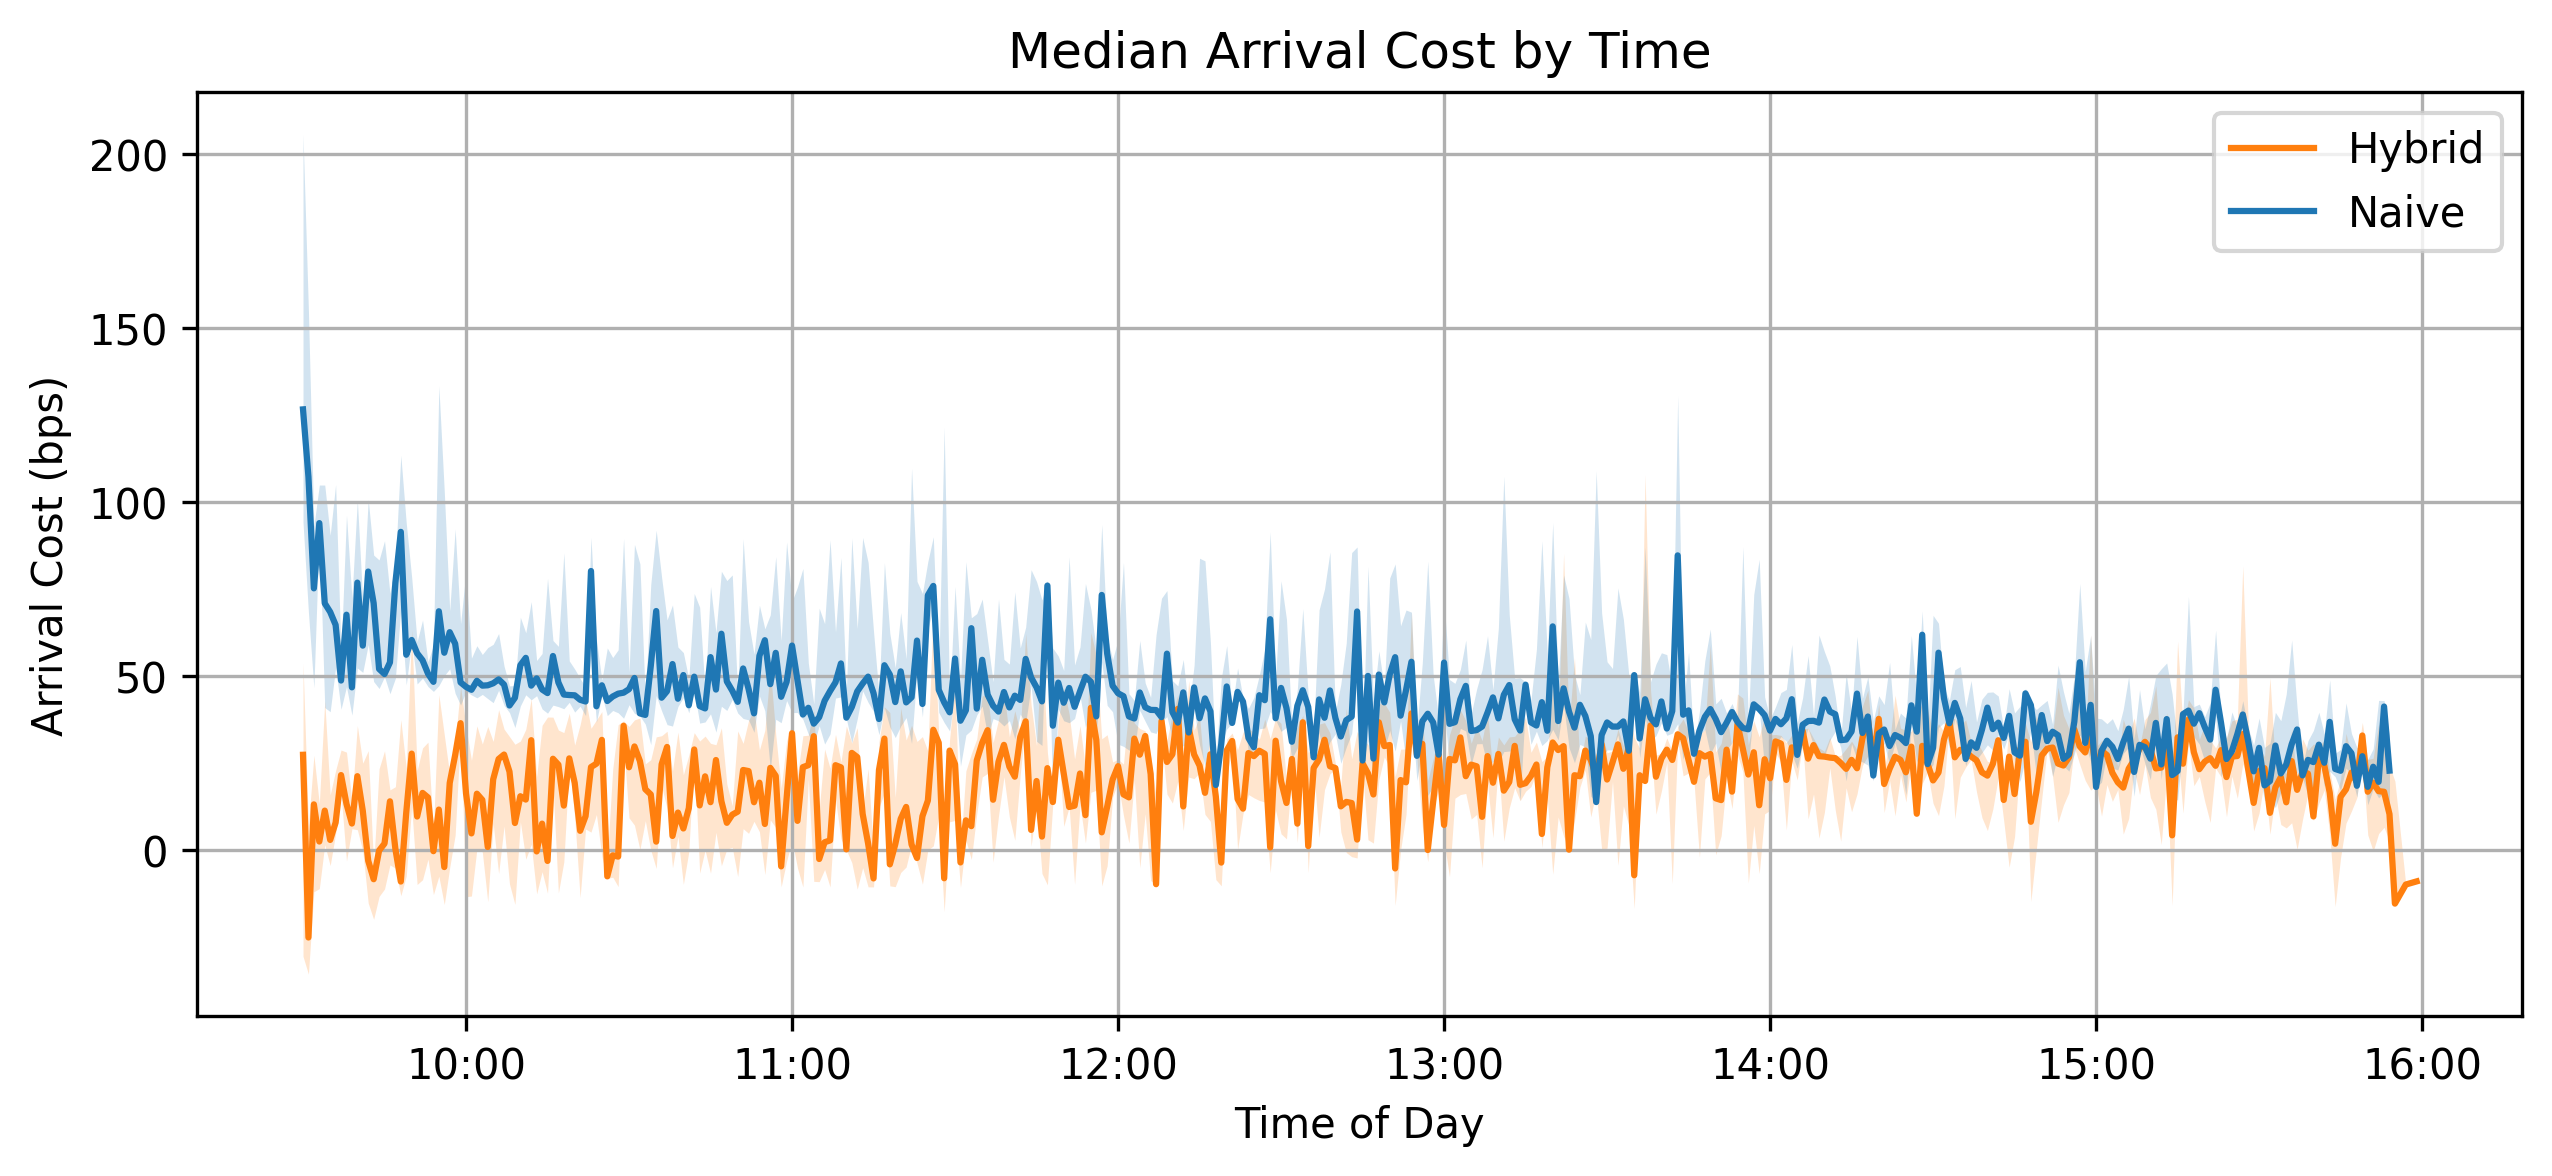
\includegraphics[width=0.52\linewidth,height=\textheight,keepaspectratio]{plots_and_data/section_3/successful_run/plots/time_mid.DRH.png}

}

\subcaption{\label{fig-time-drh}DRH}

\end{minipage}%

\caption{\label{fig-time}Intraday Seasonality of Arrival Cost}

\end{figure}%

\section{Future Work}\label{sec-future}

Overall, the imbalance calibrated aggression strategy is a highly
effective one. As always though, a few tweaks stand out in their
potential to improve upon these results. Each is laid out below.

\subsection{EMA of Book Imbalance}\label{ema-of-book-imbalance}

To prevent temporary peaks in book imbalance from affecting the
strategy's aggression, the strategy could use a moving average of book
imbalance. This would smooth the peaky nature of OBI. However, this
introduces yet more hyperparameters and is linked with the time to
expiry of resting limit orders.

\subsection{Catch-Up Mechanism}\label{catch-up-mechanism}

Currently, the strategy is placing naive IOC orders when OBI is not
strongly indicating the direction of price drift, which can cause
unnecessary price impact. This could be improved by implementing a
mechanism to measure how ahead or behind the strategy is in its filled
quantity and dynamically tweak the OBI thresholds or size of fills.

\subsection{Horizon as a Function of
Volume}\label{horizon-as-a-function-of-volume}

Currently the hybrid strategy uses a set hyperparameter for the parent
order's horizon to fill. This could be dynamically chosen as a function
of the share or dollar volume in the past few minutes, indicating how
much impact the fills are likely to have. With more volume being traded,
the time horizon can be shorter and vice-versa.

\subsection{Improving Book Simulation}\label{improving-book-simulation}

Calibrating hyperparameters like the poisson rate of replenishment would
help achieve more accurate results. Access to proprietary trading data
would also inform the choice of distribution for limit order
replenishment and sizes, as a Poisson distribution is a relatively
simple approximation.

\newpage{}

\section{Definitions and Appendix}\label{sec-definitions}

Throughout this work we refer to a few concepts that require specific
definitions. We lay them out below for reference.

\begin{itemize}
\item
  OBI: We define order book imbalance (OBI) using the top \emph{six}
  levels of the book, as follows:
  \begin{equation}\phantomsection\label{eq-obi}{
  \begin{split}
  OBI = \frac{\Sigma_{i=0}^5 [Q_{i}^{bid} - Q_{i}^{ask}]}{\Sigma_{i=0}^5 [Q_{i}^{bid} + Q_{i}^{ask}]}\in [-1, 1]
  \end{split}
  }\end{equation}
\item
  Price Impact : When referring to price impact we include only the
  mechanical impact of taking liquidity from the limit order book. Our
  order book simulation is discussed in Section~\ref{sec-sim}, and
  includes further information on impact as well as replenishment and
  latency.
\item
  Arrival Cost: When discussing to the arrival cost of a parent or child
  order, we are referring to the volume-weighted average price of a fill
  minus the mid price at the time of execution, divided by mid price and
  converted to bps. For a parent order, the VWAP sums over child order's
  individual vwaps in the same way, and the mid price is set to the
  price at the time the parent order was sent to the execution engine.
  Below, \(q_i\) and \(p_i\) are the individual fill's quantities and
  prices respectively. \begin{equation}\phantomsection\label{eq-vwap}{
  \begin{split}
  p_{vwap} &= \frac{\Sigma_{i=0}^nq_i\,p_i}{\Sigma_{i=0}^nq_i}\\ 
  \text{ArrivalCost (bps)} &= \frac{p_{vwap} - p_{mid}}{p_{mid}} * 10^4
  \end{split}
  }\end{equation}
\end{itemize}

Discussed in Section~\ref{sec-sim}, each simulated individual fill
returns a dictionary of fill statistics, below.

\begin{Shaded}
\begin{Highlighting}[]
\NormalTok{\{}\StringTok{\textquotesingle{}vwap\textquotesingle{}}\NormalTok{: }\FloatTok{211.9365352112676}\NormalTok{,}
 \StringTok{\textquotesingle{}fills\textquotesingle{}}\NormalTok{: [(}\FloatTok{211.93}\NormalTok{, }\DecValTok{246}\NormalTok{), (}\FloatTok{211.94}\NormalTok{, }\DecValTok{464}\NormalTok{)],}
 \StringTok{\textquotesingle{}total\_filled\textquotesingle{}}\NormalTok{: }\DecValTok{710}\NormalTok{,}
 \StringTok{\textquotesingle{}levels\_swept\textquotesingle{}}\NormalTok{: }\DecValTok{1}\NormalTok{,}
 \StringTok{\textquotesingle{}executed\_at\_ns\textquotesingle{}}\NormalTok{: }\DecValTok{1774538471626080001}\NormalTok{,}
 \StringTok{\textquotesingle{}arrival\_cost\textquotesingle{}}\NormalTok{: }\FloatTok{0.02153521126757596}\NormalTok{\}}
\end{Highlighting}
\end{Shaded}

\section{References}\label{references}

\begin{itemize}
\tightlist
\item
  Bouchaud, J. P., Farmer, J. D., \& Lillo, F. (2009). How markets
  slowly digest changes in supply and demand. \emph{Handbook of
  Financial Markets}.
\item
  Cont, R., Kukanov, A., \& Stoikov, S. (2014). The price impact of
  order book events. \emph{Journal of Financial Econometrics}.
\item
  Said, E. (2022). Market Impact: Empirical Evidence, Theory and
  Practice. \emph{arXiv preprint}.
\item
  Sato, Y., \& Kanazawa, K. (2024). Online Learning of Order Flow and
  Market Impact with Bayesian Change-Point Detection Methods.
  \emph{arXiv preprint}.
\item
  Obizhaeva, A. A., \& Wang, J. (2013). Optimal trading strategy and
  supply/demand dynamics. \emph{Journal of Financial Markets}, 16(1),
  1--32.
\item
  Gârleanu, N., \& Pedersen, L. H. (2013). Dynamic trading with
  predictable returns and transaction costs. \emph{Journal of Finance},
  68(6), 2309--2340.
\end{itemize}




\end{document}
